% 指定来源: arXiv:2605.26733v1, 2026-05-26. CC BY 4.0.
% 完整中文译稿;以项目book目录为编译工作目录;来源对应见coverage.json.
\originalchapter{循环语言模型的动力学稳定性}\label{stars-paper}
\begin{center}
{\bfseries 稳定循环语言模型的递归动力学, 实现可扩展的测试时潜在推理}\par
Stabilizing Recurrent Dynamics for Test-Time Scalable Latent Reasoning in Looped Language Models\par
Xiao-Wen Yang, Zi-Yu Han, Xi-Hua Zhang, Wen-Da Wei, Jie-Jing Shao, Lan-Zhe Guo, Yu-Feng Li
\end{center}
Xiao-Wen Yang 与 Zi-Yu Han 共同贡献. 作者机构为南京大学计算机软件新技术全国重点实验室、人工智能学院和智能科学与技术学院; 通讯作者 Yu-Feng Li, \texttt{liyf@nju.edu.cn}. 原文标示发表于第 43 届国际机器学习大会(ICML 2026), 本译稿对应 2026 年 5 月 26 日 arXiv v1.

\begin{remark}
本稿由 ai-self-study contributors 机器辅助翻译, 不是作者或机构的官方中文版本. 原论文及作者图件按 CC BY 4.0 署名使用, 许可为 \url{https://creativecommons.org/licenses/by/4.0/}, 原文为 \url{https://arxiv.org/abs/2605.26733v1}. 修改包括中文翻译、项目固定排版、统一引用前缀与分开的译者核查注. 图中原英文标签保留, 图注另附中文说明. 后文“我们”均指原论文作者, 作者实验并非本项目复现; 原文理论论证不等于对答案语义正确性的证明.
\end{remark}

\originalsection{摘要}\label{stars-abstract}
循环语言模型(Looped Language Models, LoopLMs)通过深度递归实现高效的潜在推理, 却表现出不可靠的测试时扩展行为: 性能常在某个迭代深度达到峰值, 随后继续循环时崩溃. 通过潜在动力学分析, 我们发现现有架构和策略在稳定性与有效性之间存在内在权衡. 将推理理解为不确定性的降低, 我们提出, 在保持有效性的同时收敛到稳定不动点, 是一个有希望的方向.

为此, 我们提出 STARS(STAbility-driven Recurrent Scaling, 稳定性驱动的循环扩展), 一个约束潜在状态趋向渐近稳定不动点的训练框架. 框架通过高效的 Jacobian 谱半径正则化与随机循环采样实现. 作者将其目标表述为在确保严格稳定性的同时最大化有效性. 算术任务实验显示, STARS 实现了可靠的测试时扩展; 在复杂数学推理中, 它显著缓解了随着循环深度增加而出现的性能退化, 并提高了峰值性能. 代码见 \url{https://github.com/njuyxw/STARS}.

\originalsection{引言}\label{stars-sec-1}
通过测试时扩展增强大语言模型(LLM)的复杂推理能力, 即在推断期间分配额外计算资源, 已成为重要研究方向\cite{stars-zhang2024llm,stars-zhang2025survey}. 主流方式依赖生成大量输出, 通常采用思维链推理\cite{stars-wei2022chain}, 或采样多个候选解并选择最优者\cite{stars-wang2022selfconsistency,stars-tot}. 近来, 循环语言模型\cite{stars-geiping2025scaling,stars-zhu2025scaling}受到关注, 被视为有希望的替代范式. 它们通过共享参数的深度递归, 模拟类似人类的潜在推理过程\cite{stars-zhu2025survey}. 其优点包括更高的计算效率: 推断时增加推理投入不必延长上下文窗口. 连续潜在表示还可能比离散 token 提供更高的信息带宽. 理想情况下, 这种架构能够在不增加参数量的前提下扩展测试时推理, 随循环次数增加逐渐精炼潜在表示\cite{stars-geiping2025scaling}.

\begin{figure}[htbp]
\centering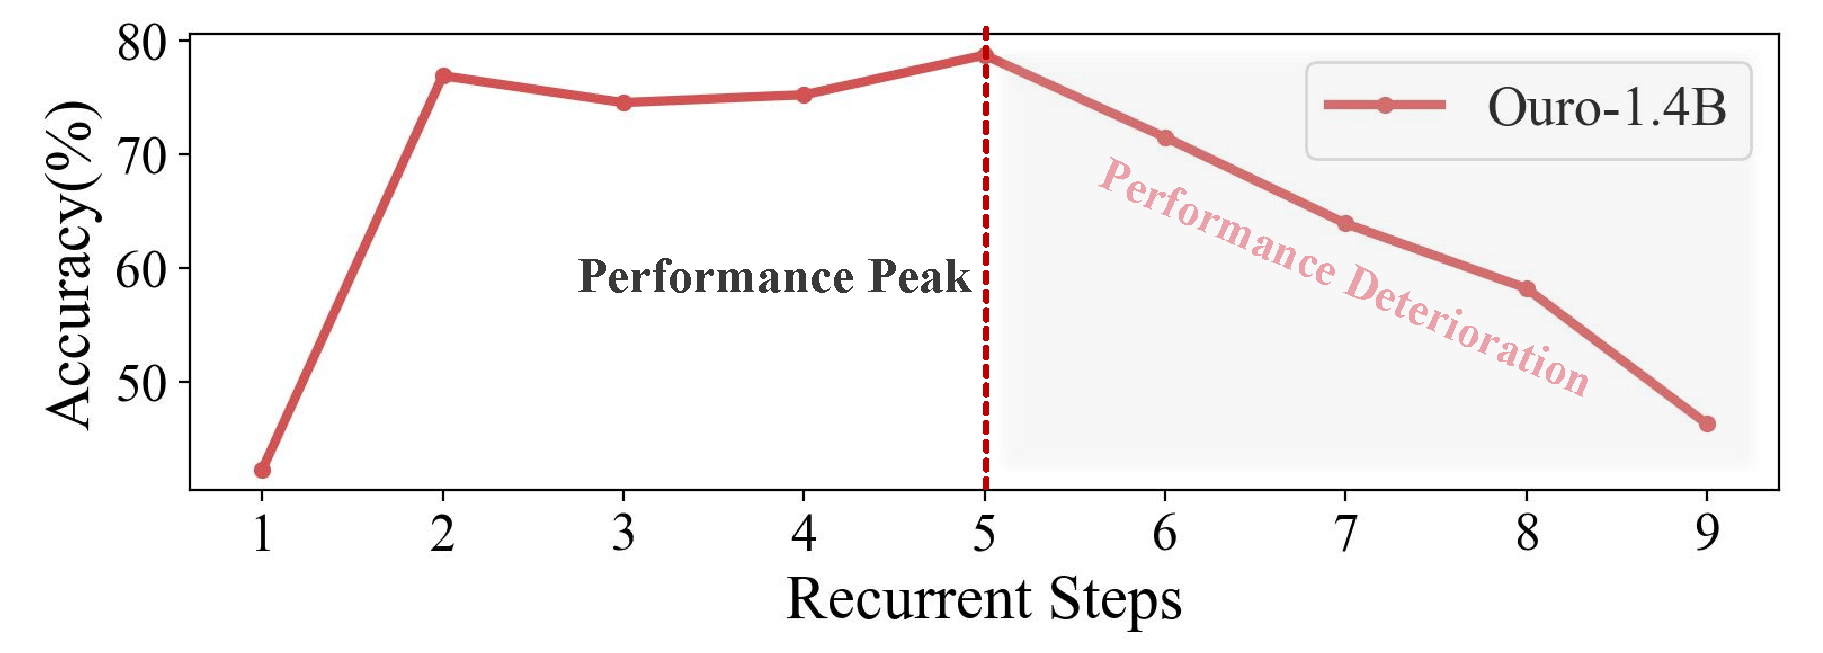
\includegraphics[width=.78\textwidth]{../papers/translations/stars/figures/intro.pdf}
\caption{原文图 1: Ouro-1.4B\cite{stars-zhu2025scaling}在 GSM8K 上随循环步数变化的性能. 图内 Accuracy 表示准确率, Recurrent Steps 表示循环步数; Performance Peak 为性能峰值, Performance Deterioration 为性能退化. 图中曲线仅为 Ouro-1.4B.}\label{stars-fig-1}
\end{figure}

然而, 我们的研究表明, 若设计不当, 当前 LoopLM 往往出现\textbf{不可靠的扩展行为}. 实验发现, 额外计算没有带来逐步改善: 性能常在某个迭代深度达到峰值, 随后循环继续增加时急剧下降, 甚至完全崩溃(图 \ref{stars-fig-1}). 这表明直接监督微调不能让模型获得通过深度递归进行测试时扩展推理的能力; 模型反而倾向于过拟合训练时特定的循环次数.

为解释这些扩展失败, 我们从动力系统视角系统诊断 LoopLM 的潜在轨迹. 分析揭示了当前设计中一个基本但先前被忽略的有效性与稳定性权衡, 作者称这一权衡在现有设计中难以调和. 我们发现, 潜在轨迹的稳定性主要由归一化的位置决定. 内部归一化, 如 Pre-Norm, 维持信息流, 即有效性, 但使隐状态指数增长并导致轨迹发散. 相反, 外部归一化, 如 Post-Norm, 保证状态有界, 即稳定性, 却常不能完成深层推理. 我们的实验显示, 辅助 Prelude/Coda 层、L2 正则化和随机循环采样等常见补救措施, 均不能完全解决这一僵局.

本文的一个关键观点是, 可在测试时扩展的潜在推理必须同时满足有效性和稳定性. 我们认为推理是反复降低不确定性、精炼思考的过程. 从动力学看, 隐状态应当收敛到有效且稳定的不动点. 有效但不稳定的系统会产生混乱的推理轨迹; 稳定但无效的系统则产生浅层思考. 为实现这一目标, 我们提出统一训练框架 STARS, 将 Jacobian 谱半径正则化(JSRR)与随机循环采样结合. 根据 Lyapunov 线性化定理, 非线性系统的稳定性由其 Jacobian 谱半径决定. 作者据此主张, STARS 在训练中限制该谱半径, 从数学上驱动模型趋向渐近稳定不动点.

为让框架适用于大规模 LLM, 我们避免成本过高的直接特征值计算. STARS 将单步幂迭代与 Jacobian--向量积(JVP)结合, 采用轻量高效的估计方案. 通过随机循环采样, STARS 在全局尺度上优化潜在轨迹的有效性与稳定性, 以获得更稳健的测试时扩展.

我们使用两种实验设置评价方法: 在随机初始化的 Transformer 上完成基础算术任务\cite{stars-vaswani2017attention}, 以及在复杂数学推理任务上微调预训练 LoopLM. 算术结果显示, 方法实现了完全可靠的测试时扩展; 数学推理结果显示, 相比基线具有更稳健的性能. 例如在 GSM8K 上, 循环到 8 步时, Ouro-1.4B 相比峰值下降 $20.47\%$, 而我们的方法仅下降 $8.26\%$. 同时, 方法在 GSM8K 上将峰值性能提高了 $4.01\%$.

\originalsection{相关工作}\label{stars-sec-2}
\noindent\textbf{测试时扩展与潜在推理.}
测试时计算扩展是增强 LLM 推理能力的重要前沿\cite{stars-zhang2025survey}. 传统方法主要依赖显式推理, 即生成自然语言中间步骤, 例如思维链提示\cite{stars-wei2022chain}, 来求解复杂任务. 多数投票\cite{stars-wang2022selfconsistency}、思维树(ToT)\cite{stars-tot}以及蒙特卡洛树搜索(MCTS)\cite{stars-yang2022chain}等搜索策略能够探索多条推理路径, 带来进一步改善. 但这些方法仍受自然语言生成的带宽和效率限制.

受人类倾向于先在内部推理、而非立即输出语言的现象启发\cite{stars-zelikman2024quiet}, 近期工作转向潜在推理, 将计算从离散 token 移到潜在表示\cite{stars-zhu2025survey}. 作者认为这种方式更有效率, 也更适合抽象推理. Coconut\cite{stars-hao2024training}是典型方法, 使用从先前隐状态得到的连续思考 token. SIM-CoT\cite{stars-wei2025sim}及其他方法\cite{stars-mohtashami2023cotformer,stars-shen2025codi,stars-cheng2024compressed,stars-zhang2025lightthinker}也采用相似思路. 不过, 这些方式本质上仍沿序列维度扩展测试时计算.

\noindent\textbf{循环 Transformer 与 LoopLM.}
与扩展序列长度的方法不同, 较新的潜在推理范式通过递归与参数共享扩展模型深度. Universal Transformer\cite{stars-dehghani2018universal}率先探索跨层动态递归, 将深度自适应计算作为固定深度 Transformer 的替代. 随后的研究\cite{stars-giannou2023looped,stars-yang2023looped,stars-fan2024looped}通过理论与小规模实验分析其潜在优势.

近期工作\cite{stars-geiping2025scaling,stars-zhu2025scaling,stars-du2025latent,stars-mcleish2025teaching}已把循环 Transformer 扩展到语言模型. Huginn\cite{stars-geiping2025scaling}从头训练了一个 3.5B 模型; Ouro\cite{stars-zhu2025scaling}提出能力更强的 LoopLM, 可以与主流开放 LLM 竞争. 作为典型潜在推理方法, LoopLM 本应呈现测试时扩展. 然而, 我们发现, 计算增加往往不带来持续收益, 性能通常在特定迭代深度达到峰值, 之后急剧下降; Ouro 模型中这一现象尤其明显.

现有研究对 LoopLM 训练设计缺乏深入分析, 尤其缺少潜在动力学分析. 虽然深度平衡模型(DEQ)\cite{stars-bai2019deep,stars-bai2021stabilizing}研究了循环网络的动力学, 其架构和训练算法与标准语言模型不同. 因而, 研究现代 LoopLM 的潜在动力学, 对解决不可靠扩展行为十分重要.

\originalsection{预备知识}\label{stars-sec-3}
\noindent\textbf{循环语言模型.}\label{stars-sec-3-1}
传统深层架构堆叠不同层, 循环语言模型则共享权重, 反复应用循环模块 $\mathcal M^L$. 架构定义为
\[
\mathcal F^{(t)}(\cdot)=\operatorname{lmhead}\circ\operatorname{coda}\circ
\underbrace{\mathcal M^L\circ\cdots\circ\mathcal M^L}_{t\text{ 次迭代}}\circ\operatorname{prelude}(\cdot),
\]
其中 $\circ$ 表示函数复合, 各组件如下:
\begin{itemize}
\item $\operatorname{prelude}:\R^{M\times|V|}\to\R^{M\times d}$ 把包含 $M$ 个 token 的序列映射为 $d$ 维 embedding, 作为输入文本预处理.
\item $\mathcal M^L:\R^{M\times d}\to\R^{M\times d}$ 表示 $L$ 个隐层维度为 $d$ 的因果 Transformer 层堆叠, 即 $\mathcal T_{\theta_L}\circ\cdots\circ\mathcal T_{\theta_1}$.
\item $\operatorname{coda}:\R^{M\times d}\to\R^d$ 将最终迭代表示变换为输出层使用的表示.
\item $\operatorname{lmhead}:\R^d\to\R^{|V|}$ 将输出投影回大小为 $V$ 的词表以生成 token.
\end{itemize}
特殊情况 $t=1$ 时, 架构退化为标准非循环模型 $\mathcal F^{(1)}\equiv F$. 对训练批次 $\mathcal D=\{\mathbf x^{(i)}\}_{i=1}^N$, 定义 $t$ 次迭代时的标准交叉熵损失为
\begin{equation}\label{stars-eq-1}
\mathcal L_{\rm SFT}^{(t)}=\frac1N\sum_{i=1}^N\sum_{\ell=1}^{M_i-1}
-\log p_\theta^{(t)}(x_{\ell+1}^{(i)}\mid x_{1:\ell}^{(i)}).
\end{equation}
条件概率为 $p_\theta^{(t)}(\cdot\mid x_{1:\ell})=\softmax(\operatorname{lmhead}(h_\ell^{(t)}))$. 这里 $x_{1:\ell}$ 是长度为 $\ell$ 的前缀, $h_\ell^{(t)}$ 是递归迭代 $t$ 次后位置 $\ell$ 的隐状态.

\noindent\textbf{作为动力系统的潜在推理.}\label{stars-sec-3-2}
LoopLM 的迭代计算自然地在潜在空间中定义一个离散时间动力系统. 对给定输入 $\mathbf x$, 初始 embedding 之后的循环变换产生如下演化:
\begin{equation}\label{stars-eq-2}
\mathbf h^{(t+1)}=\Phi_\theta(\mathbf h^{(t)}),\qquad t=0,1,2,\ldots.
\end{equation}
其中 $\mathbf h^{(t)}\in\R^D$, $D=M\cdot d$, 是第 $t$ 次迭代展平后的潜在状态; $\Phi_\theta:=\mathcal M^L$ 是由 $\theta$ 参数化的确定性非线性映射. 轨迹是序列 $(\mathbf h^{(0)},\mathbf h^{(1)},\ldots)$. 从这个视角看, 测试时扩展是增加系统轨迹长度, 在参数不变的前提下增加迭代次数 $t$. 扩展能否成功, 因而取决于轨迹的长期行为.

\noindent\textbf{吸引子与不动点.}\label{stars-attractors}
动力系统理论中, 吸引子描述系统的长期演化. 形式上, 若集合 $\mathcal A\subset\R^D$ 存在邻域 $\mathcal U\supset\mathcal A$, 使每个处于 $\mathcal U$ 的状态 $\mathbf h^{(t)}$ 满足
\[
\lim_{t\to\infty}\operatorname{dist}(\mathbf h^{(t)},\mathcal A)=0,
\]
则 $\mathcal A$ 是 $\Phi_\theta$ 所诱导动力学的吸引子. $\operatorname{dist}(\cdot,\mathcal A)$ 表示到集合 $\mathcal A$ 的距离. 直观上, 吸引子是模型内部表示在推理时趋向的潜在空间区域.

不动点是一类特别重要的吸引子. 状态 $\mathbf h^\star\in\R^D$ 若满足 $\Phi_\theta(\mathbf h^\star)=\mathbf h^\star$, 就是不动点. 潜在轨迹到达这个状态后, 继续应用循环模块不再改变表示. 在 LoopLM 中, 作者把不动点理解为表示推理过程完成的稳定内部表示.

若存在 $\epsilon>0$, 使每个满足 $\|\mathbf h^{(t)}-\mathbf h^\star\|<\epsilon$ 的状态都有 $\lim_{t\to\infty}\mathbf h^{(t)}=\mathbf h^\star$, 则称不动点 $\mathbf h^\star$ 局部渐近稳定. 这类稳定不动点是推理任务所希望的, 因为延长推断时, 它们保证的是收敛而非振荡或发散.

\originalsection{LoopLM 的循环动力学}\label{stars-sec-4}
为了深入分析支配 LoopLM 内在动力学的核心因素, 本节开展一系列系统诊断实验. 先介绍实验设置, 再分析关键架构组件对循环模型推理不稳定性的影响, 最后探索可扩展潜在推理的候选策略.

\noindent\textbf{实验设置.}\label{stars-sec-4-1}
研究建立在使潜在动力学可观测的受控环境中. 我们将多位数加法作为分析迭代算法推理的理想化测试平台.

\noindent\textbf{任务描述.}
模型在两个四位数的加法题上训练, 例如 $1234+5678=6912$, 词表包含数字、算术运算符和特殊 token. 训练数据包含随机生成的 100,000 个样本. 作者认为这一规模足以排除机械记忆并促使模型学习可泛化的加法算法. 选择四位数加法是对计算约束与任务复杂度的折中: 两位数加法的样本空间只有 $10^4$ 种组合, 四位数则有 $10^8$ 种, 为分析提供足够复杂的空间, 对未预训练 Transformer 构成非平凡挑战.

\noindent\textbf{模型架构.}
我们使用标准 GPT 风格的 Transformer 模块\cite{stars-vaswani2017attention,stars-radford2019language}作为最小循环单元, $L=1$, 通过递归迭代该单元构成循环模型. 这一选择排除了深层异构堆叠带来的混杂, 使性能变化可以归因于同一个明确的状态转移函数被反复应用. 单元超参数为 $d_{\rm model}=512$, $n_{\rm heads}=8$, $d_{\rm ff}=1024$.

\noindent\textbf{评价细节.}
静态架构分析中, 模型按固定循环次数 $T_{\rm train}=4$ 训练. 评价时, 在较宽范围扫描测试循环次数 $T_{\rm test}$. 主要关注 $T_{\rm test}$ 偏离、尤其超过训练时域 $T_{\rm train}$ 时, 系统稳定性和内部状态轨迹怎样演化. 我们对潜在状态序列进行主成分分析(PCA), 投影到前两个主成分张成的二维空间中可视化.

\begin{figure}[p]
\centering
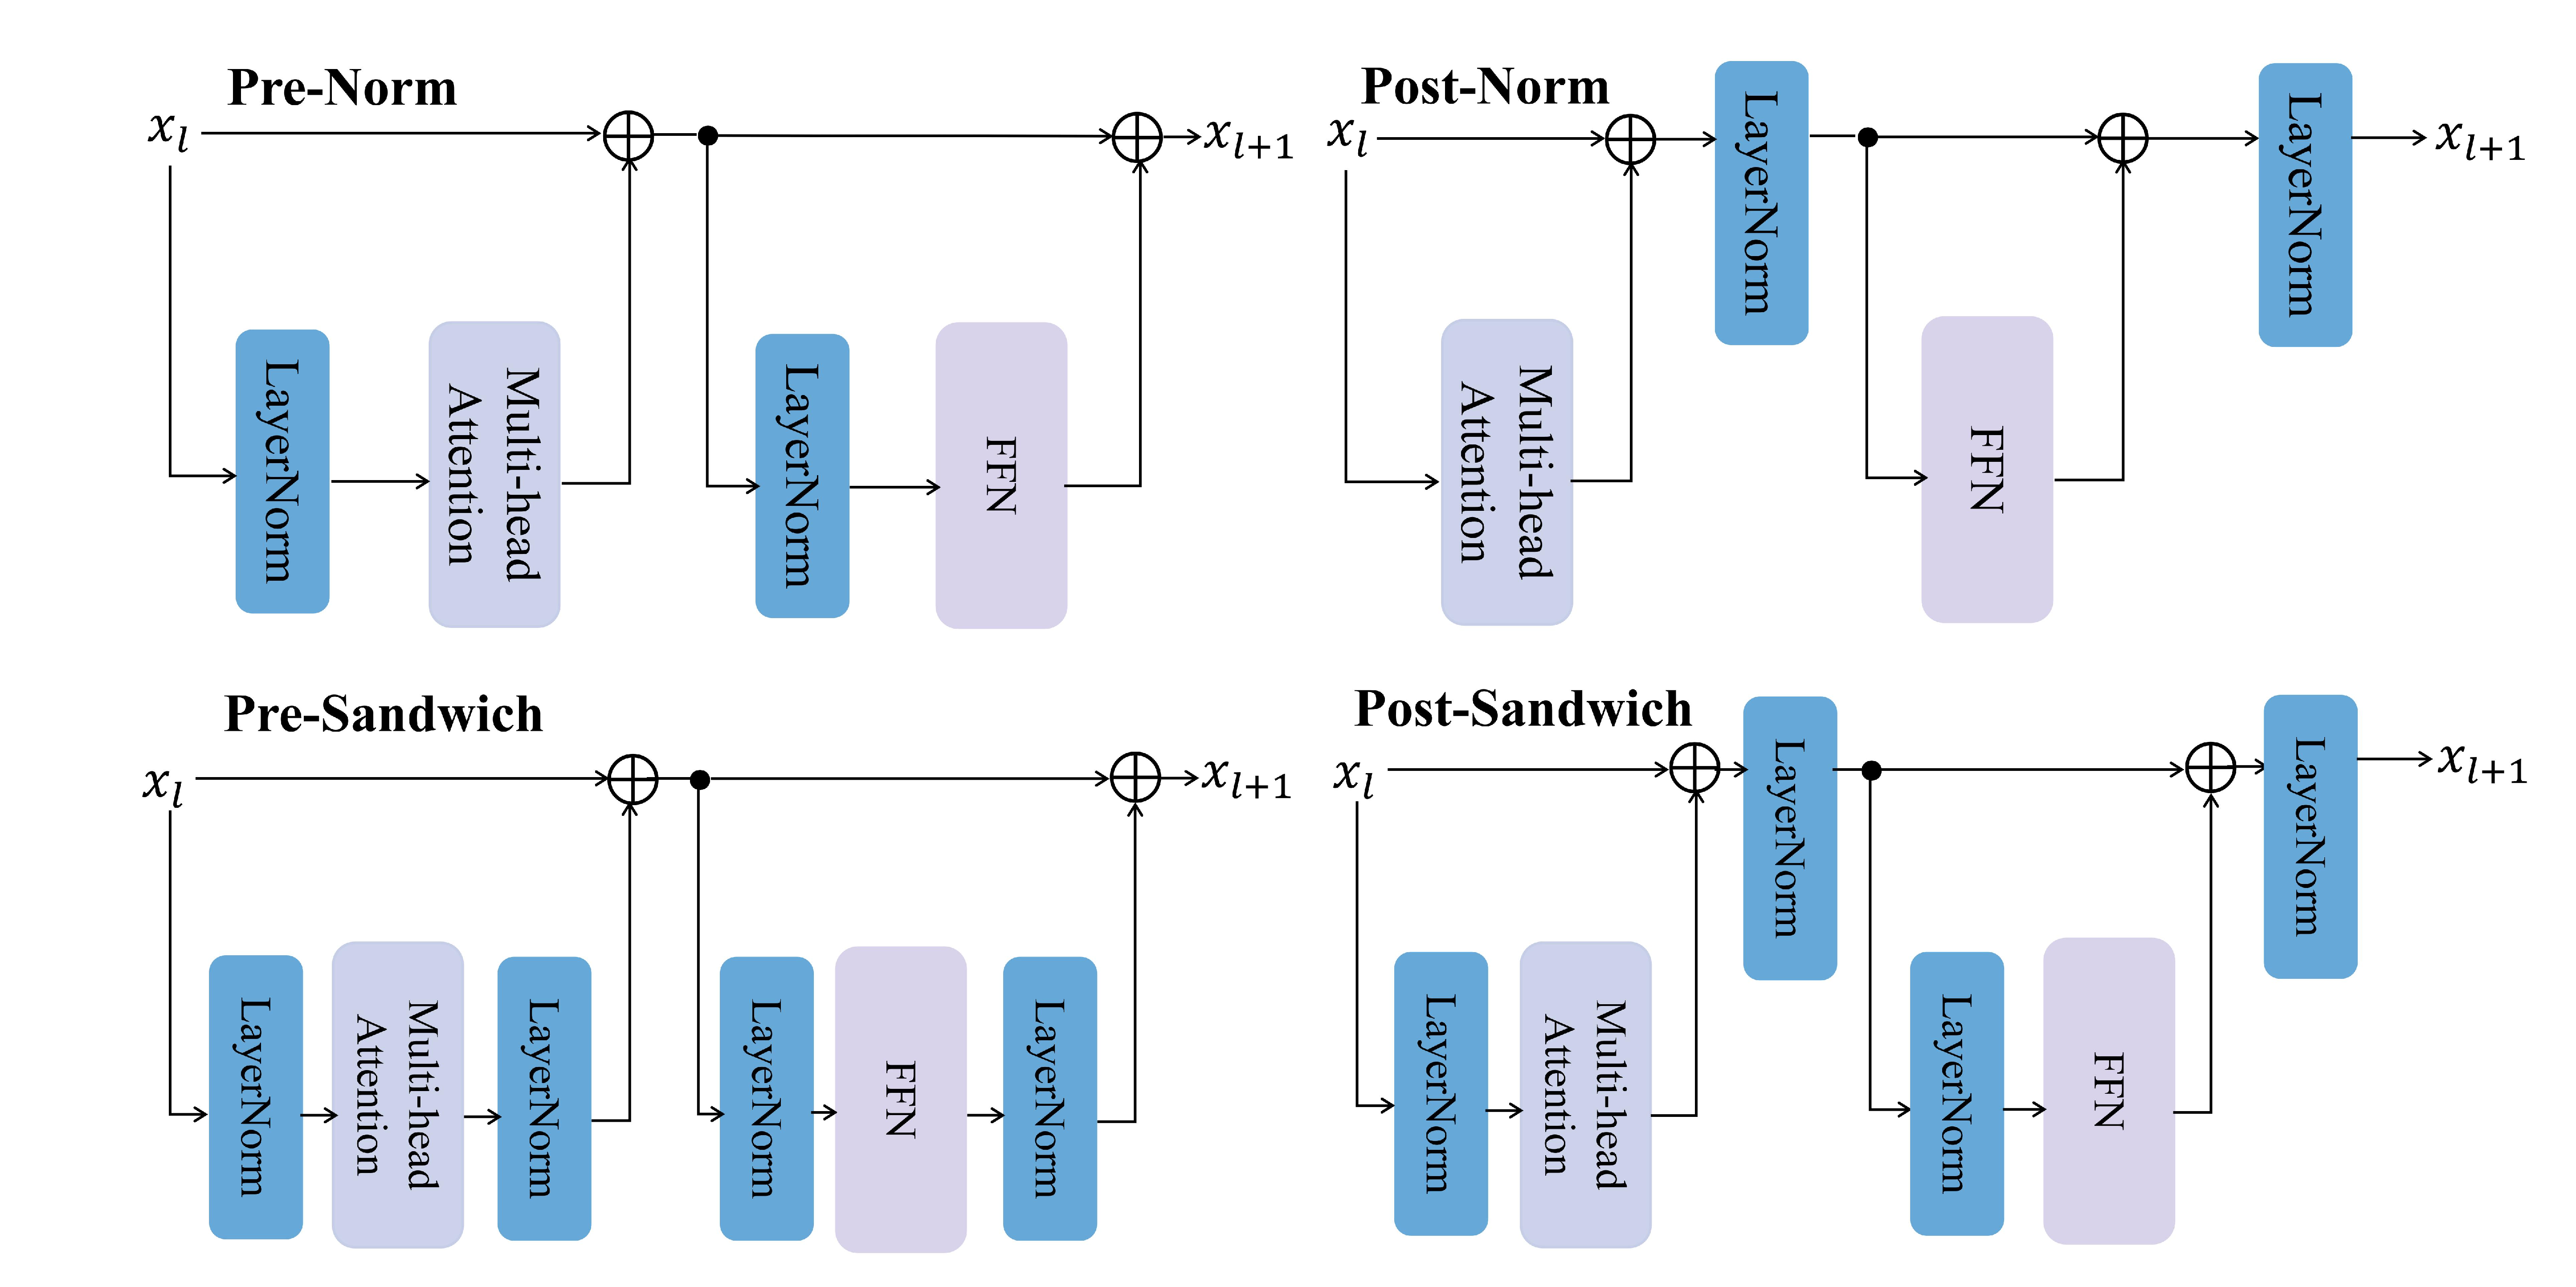
\includegraphics[width=.91\textwidth]{../papers/translations/stars/figures/norm.pdf}\par
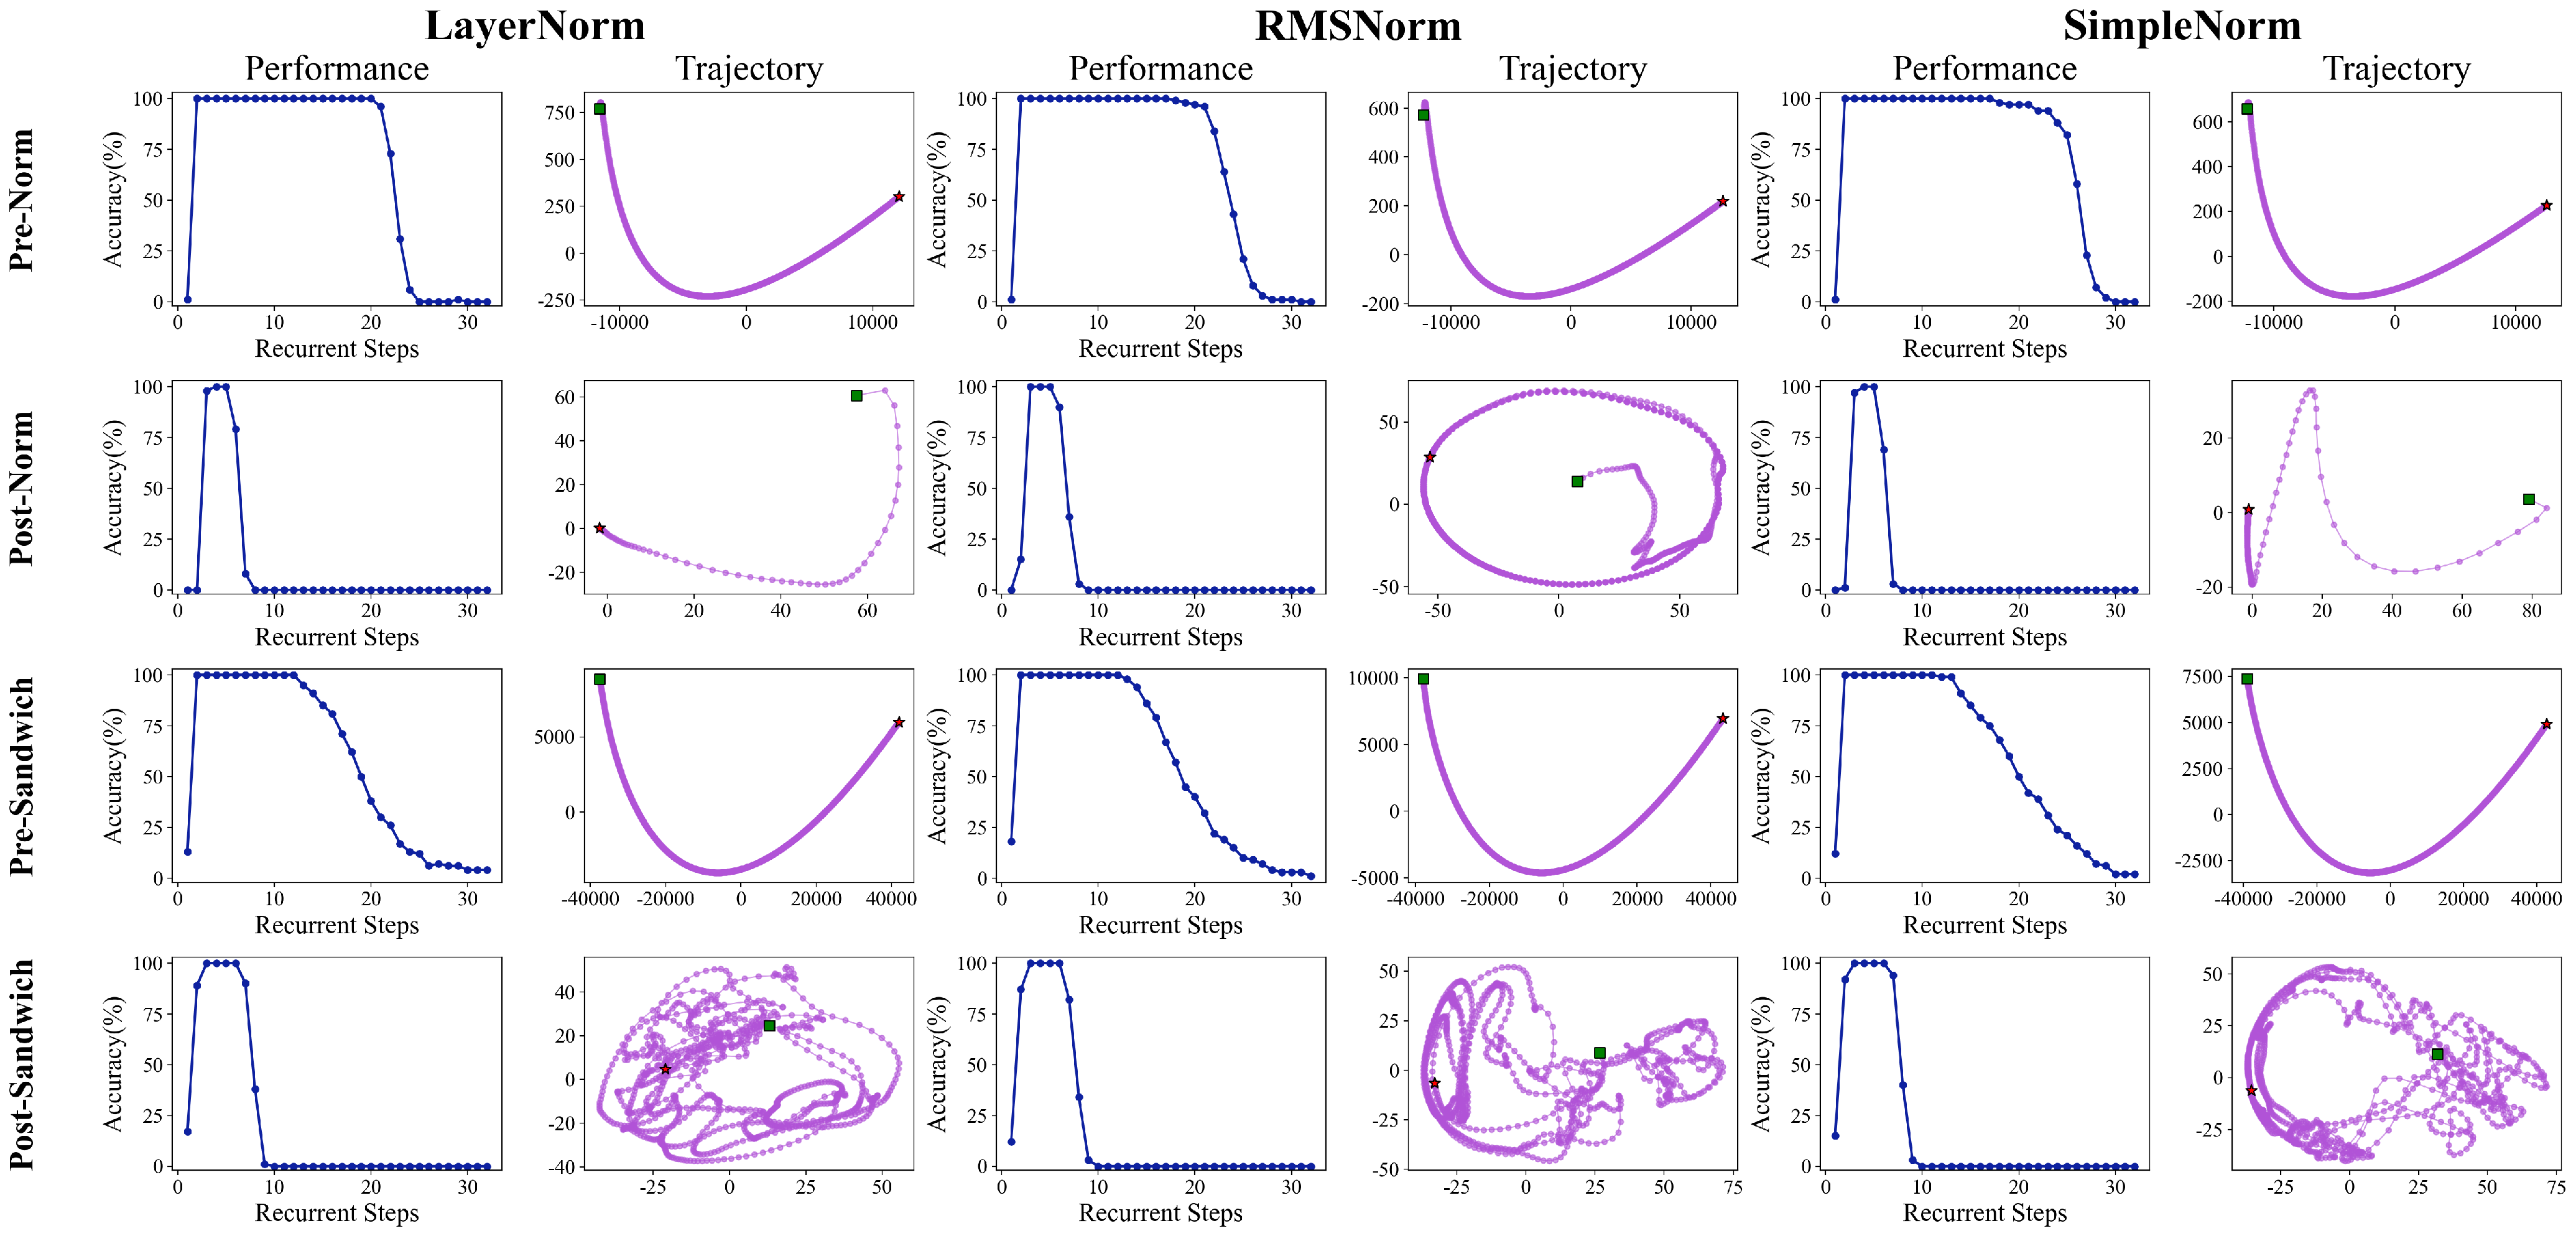
\includegraphics[width=.91\textwidth]{../papers/translations/stars/figures/norm_anal.pdf}
\caption{原文图 2: 原图左侧为结构示意, 右侧为准确率演化与潜在状态动力学可视化; 译稿将两部分上下排列. 图内 Pre/Post 分别为前置/后置归一化, Pre-Sandwich/Post-Sandwich 为两种夹心结构; Multi-head Attention 为多头注意力, FFN 为前馈网络, LayerNorm 为层归一化. LayerNorm/RMSNorm/SimpleNorm 为三种算子; Accuracy/Recurrent Steps 为准确率/循环次数, Performance/Trajectory 为性能/轨迹; 轨迹坐标表示 PCA 前两主成分.}\label{stars-fig-2}
\end{figure}

\noindent\textbf{静态架构分析.}\label{stars-sec-4-2}
循环单元的架构配置从根本上决定信息流的演化. 我们比较 Layer Normalization\cite{stars-ba2016layer}、RMSNorm\cite{stars-zhang2019root}及 SimpleNorm 三种归一化变体; SimpleNorm 定义为没有可学习仿射参数的归一化. 对每种算子, 在四种结构位置上进行比较.

\noindent\textbf{归一化结构设计的影响.}
四种位置是 Pre、Post、Pre-Sandwich 与 Post-Sandwich(图 \ref{stars-fig-2}). 选择这些位置, 主要因为既有研究发现归一化位置显著影响训练稳定性和性能\cite{stars-xiong2020layer,stars-bai2021stabilizing}. 合计得到 12 种架构组合. 按相应形式, 我们将其分成两类系统: \emph{内部归一化系统}, 即残差连接在归一化范围之外的 Pre-Norm 和 Pre-SandwichNorm; \emph{外部归一化系统}, 即残差流被最终归一化包住的 Post-Norm 和 Post-SandwichNorm.

实验显示循环 Transformer 架构中存在内在设计困境. 如图 \ref{stars-fig-2}, 具体归一化算子对潜在动力学的影响很小; 相反, 层的结构位置是决定因素, 引发两种不同失败模式.
\begin{remark}
\textbf{发现 1:} 具体归一化算子对模型动力学的影响可以忽略, 层的结构位置则决定系统的演化行为.
\end{remark}

在内部归一化系统中, 性能能维持到训练时域及其后短暂外推区间, 但随测试迭代增加而下降. PCA 轨迹尺度显著扩大, 表明隐状态逐渐漂离有效的结构流形, 最终使性能崩溃. 特别地, 在 Pre-Norm 形式 $x_{l+1}=x_l+f(\operatorname{Norm}(x_l))$ 中, 残差连接形成信息高速通路\cite{stars-he2016deep}, 将先前状态无衰减地传到下一时刻. 但更新向量 $f(\operatorname{Norm}(x_l))$ 直接累积在主干流上. 残差相加后没有约束机制, 隐状态范数便倾向于无界增长. 这形成正反馈, 状态大小随迭代线性放大, 最终偏离有效数据流形.

相反, 外部归一化系统虽然只在短暂测试区间维持性能, 潜在动力学始终有界, PCA 投影的紧凑尺度显示了这一点. 随测试迭代增加, 两类系统最终都趋向吸引子. 因此, 当前归一化架构在系统稳定性与有效信息传播之间造成权衡, 两种形式都未实现可在测试时扩展的潜在推理.
\begin{remark}
\textbf{发现 2:} 内部归一化系统允许强信息沿残差主干传播, 维持早期性能, 但可能导致不稳定及状态发散. 外部归一化系统约束残差流, 保证状态边界稳定, 却让系统落入较差状态而降低性能.
\end{remark}

\noindent\textbf{Prelude 与 Coda 层的影响.}
一个自然问题是, 像 Huginn\cite{stars-geiping2025scaling}那样在循环模块前后加入非循环层, 能否缓解这些限制. 我们在实验中加入 Prelude 和 Coda 层. 新层采用与循环单元相同的模块架构, 但不参与循环迭代.

根据具体归一化算子影响很小的发现, 这一分析固定使用 LayerNorm. 我们在 Pre-Sandwich 与 Post-Sandwich 两种结构基线上比较四项配置: 仅循环模块、加入 Prelude、加入 Coda、两者都加入.

如图 \ref{stars-fig-3}, 对内部归一化系统, 加 Prelude 只略微减缓性能下降, 影响很小; 轨迹漂移尺度依然巨大, 准确率迅速降到零. 对外部归一化系统, Coda 层虽然让最终吸引子更集中, 这些却是不良不动点, 没有带来性能收益.
\begin{remark}
\textbf{发现 3:} 加入 Prelude 和 Coda 层不改变系统的动力学趋势. 这些层可能有助于更深入地理解输入、输出空间的语义, 但对系统稳定性的影响可以忽略.
\end{remark}

\begin{figure}[p]
\centering
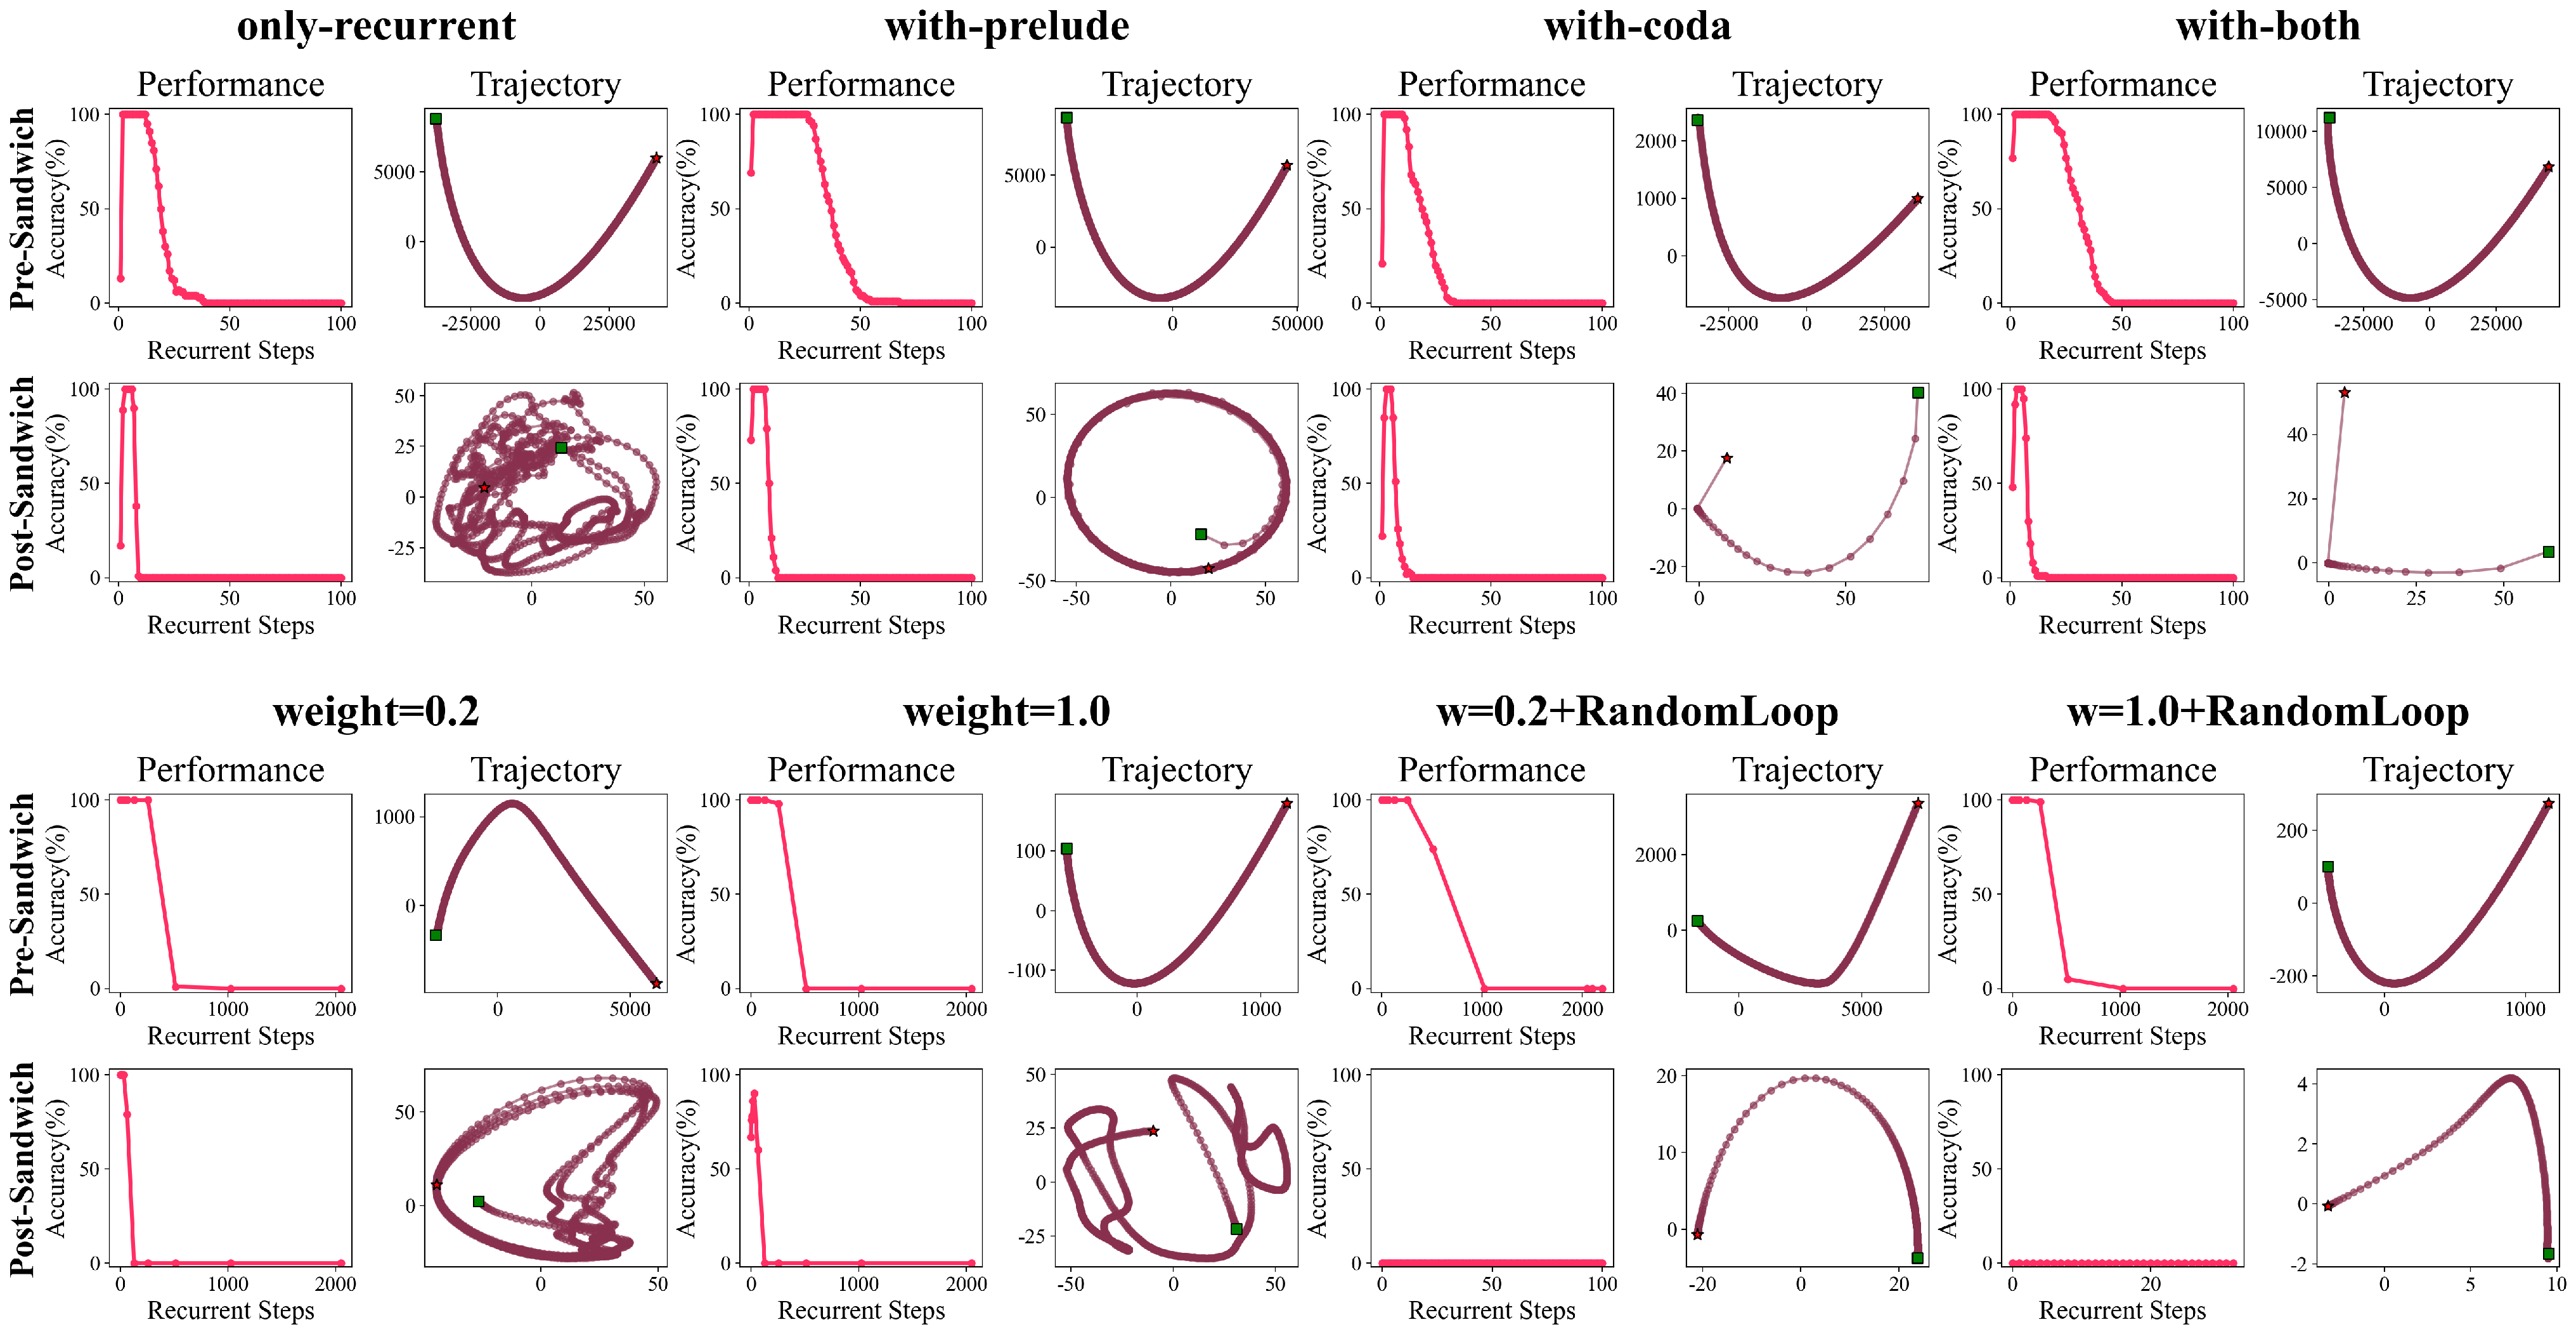
\includegraphics[width=.91\textwidth]{../papers/translations/stars/figures/prelude_coda.pdf}\par
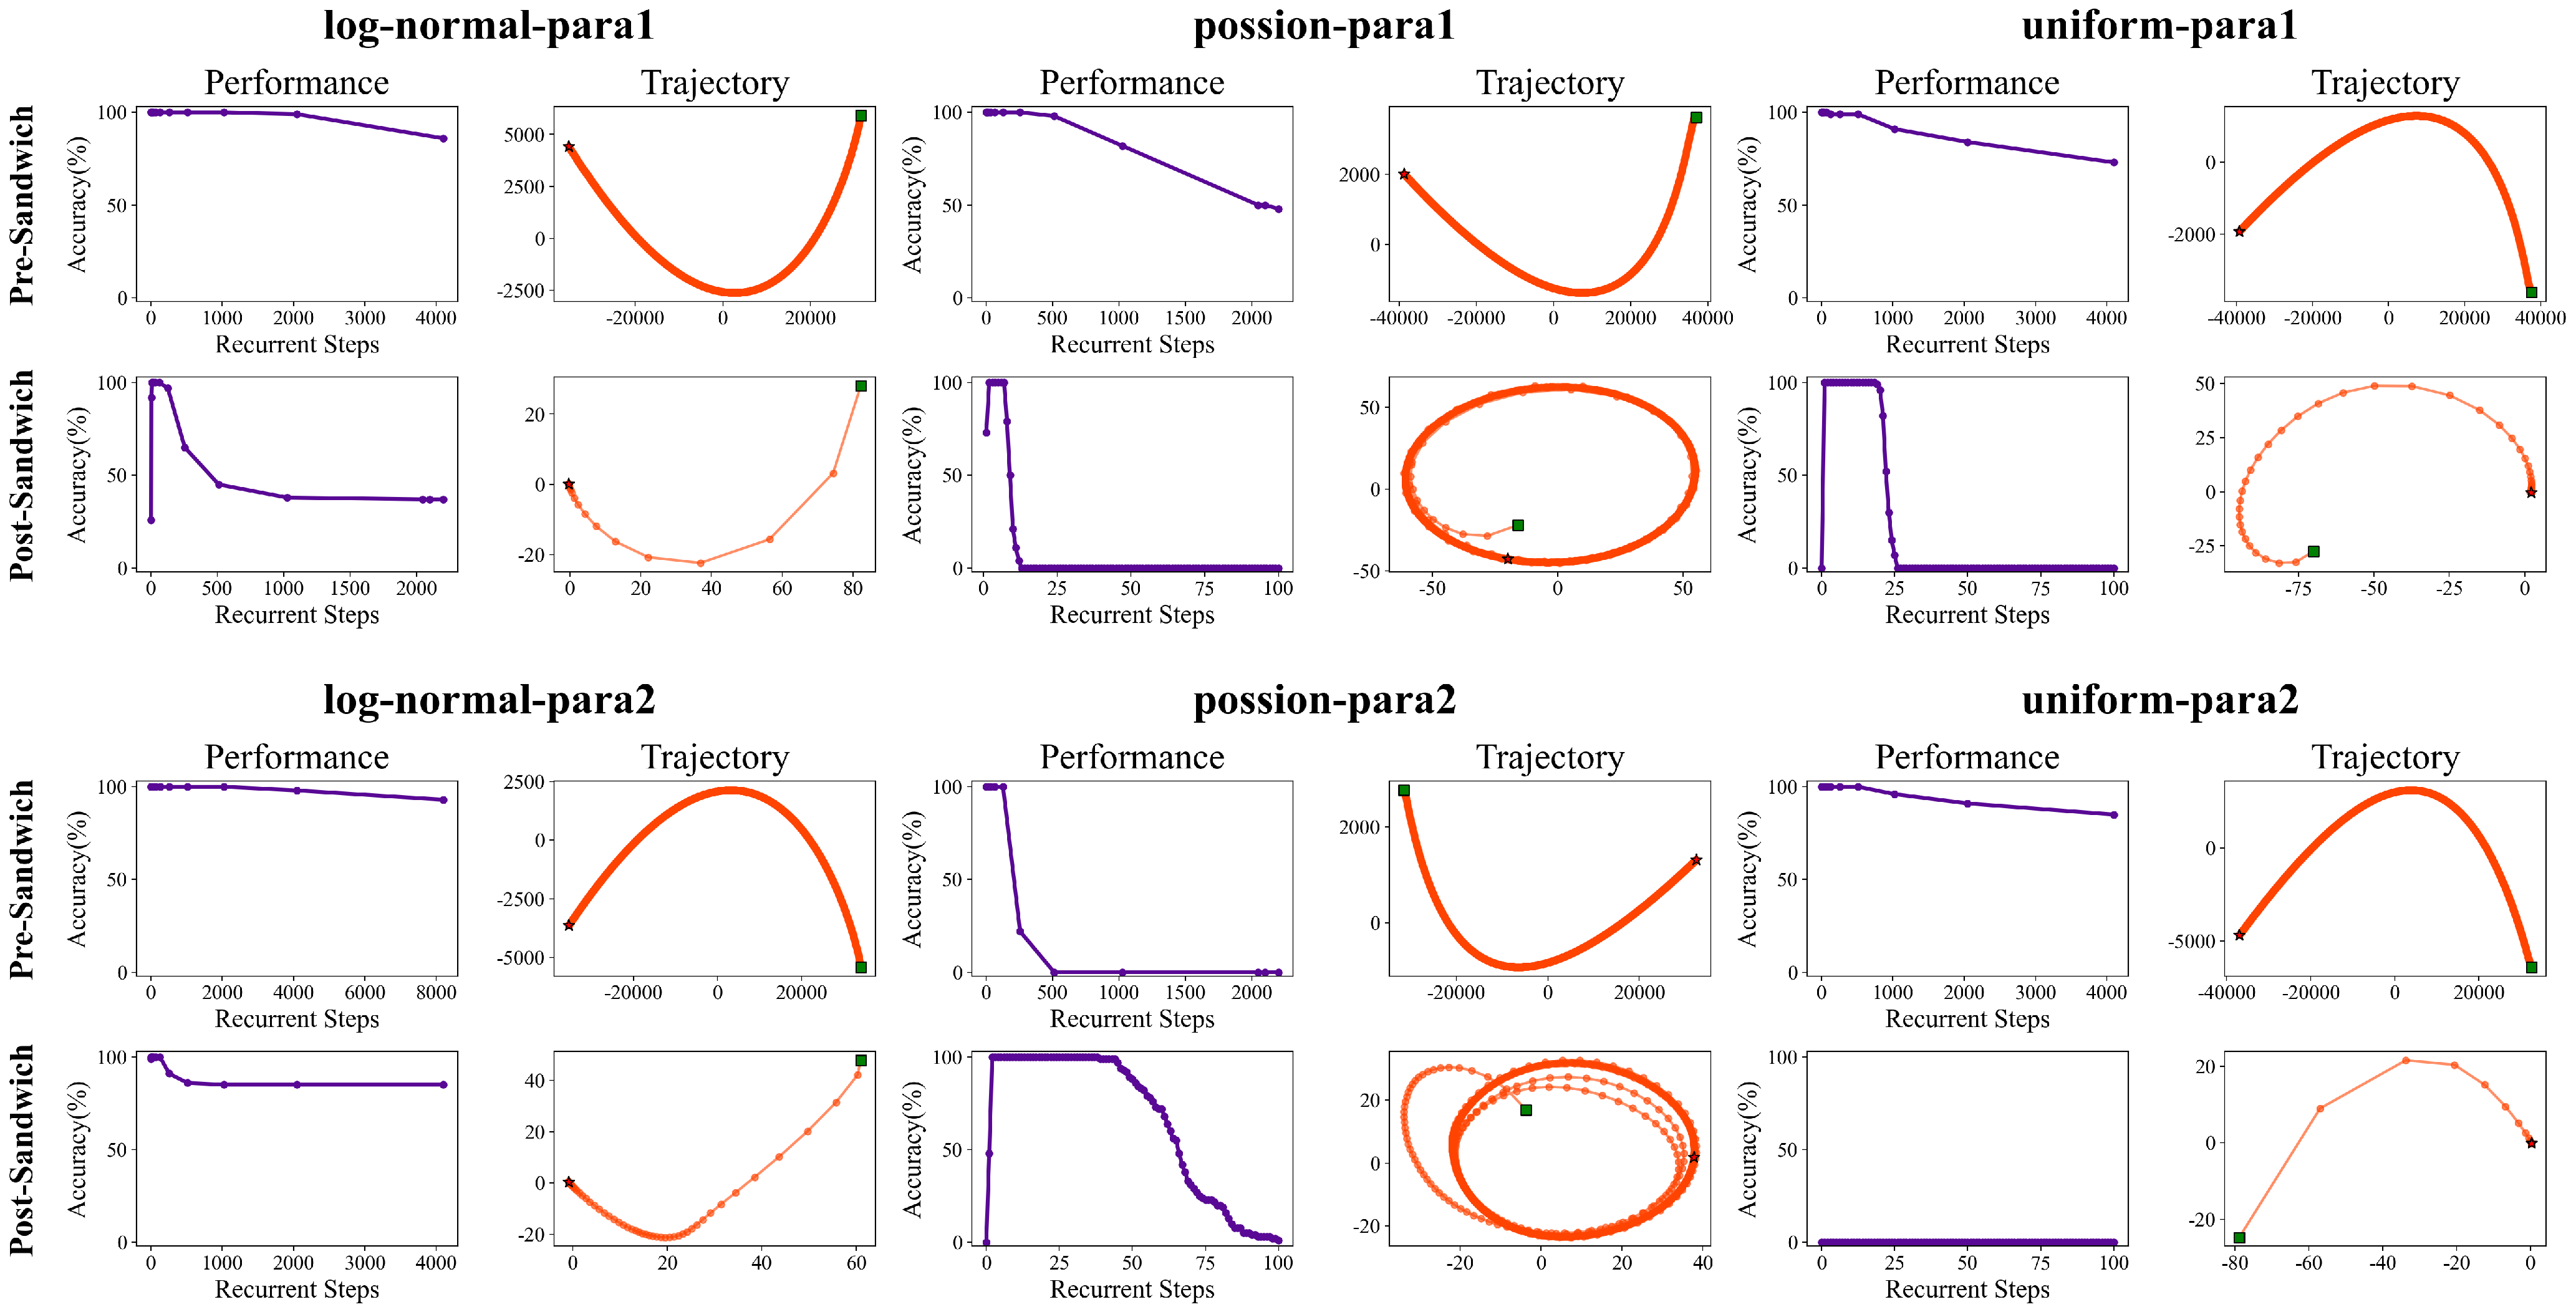
\includegraphics[width=.91\textwidth]{../papers/translations/stars/figures/random.pdf}
\caption{原文图 3: 原图左部上方分析加入非循环层的影响, 下方分析 L2 正则化; 右部分析不同分布和参数组的随机循环策略, 参数见表 \ref{stars-tab-1}. 译稿把原左右两部分上下排列. 图内 Only-Recurrent/With-Prelude/With-Coda/With-Both 分别表示仅循环/加前置层/加后置层/两者都加; L2 与 Random Loop 表示相邻状态正则和随机循环. Log-Normal/Poisson/Uniform 分别为对数正态/泊松/均匀分布; para1/para2 为参数组 1/2, weight/w 为正则权重. Performance/Trajectory 表示性能/轨迹, Accuracy/Recurrent Steps 表示准确率/循环步数. 每项展示性能变化及 PCA 状态轨迹.}\label{stars-fig-3}
\end{figure}

\begin{table}[htbp]
\centering
\caption{原文表 1: 随机循环分布的超参数. 范围是截断边界 $[\min,\max]$.}\label{stars-tab-1}
\begin{tabular}{lll}\toprule
分布 & 参数组 1 & 参数组 2\\\midrule
对数正态 & $\mu=2.62$, $\sigma=0.60$ & $\mu=2.00$, $\sigma=0.70$\\
 & 范围 $[1,40]$ & 范围 $[1,100]$\\
泊松 & $\lambda=5$ & $\lambda=10$\\
 & 范围 $[1,30]$ & 范围 $[1,30]$\\
均匀 & 范围 $[1,10]$ & 范围 $[1,40]$\\\bottomrule
\end{tabular}
\end{table}

\noindent\textbf{可扩展潜在推理的尝试方法.}\label{stars-sec-4-3}
\noindent\textbf{随机循环采样.}
随机循环采样通过为每个批次动态采样循环次数, 使性能不再绑定固定训练步数 $T_{\rm train}$. 此前循环模型训练已使用这一方法\cite{stars-geiping2025scaling}, 但没有系统分析它的影响与内在机制. 为补上这点, 我们详细研究三种分布: 对数正态、泊松和均匀; 每种有两组参数, 应用到 Pre-Sandwich 与 Post-Sandwich 两种代表架构. 其他架构结果见附录的更多结果一节.

如图 \ref{stars-fig-3}, 训练时采样迭代次数有助于维持性能. 对 Pre-Sandwich, 随机循环采样非常有效, 所有组合的性能保持范围都远超训练遇到的迭代范围. 然而, 原文随后称这没有改变“外部归一化系统”的基本性质, 状态漂移依然发生.

对 Post-Sandwich, 与先前轨迹图相比, 最终收敛的吸引子集合更紧凑, 但训练过程不稳定, 有时模型甚至无法学会任务. 从对数正态和均匀配置可见, 更大的采样范围、更高的均值不一定更好. 例如采样范围变宽时, Post-Sandwich 易训练崩溃, 学不会任务. 不过, 它本来就倾向于收敛到吸引子, 因此潜力更大. 若能引导它收敛到有效吸引子, 就有可能同时实现稳定性和有效性.
\begin{remark}
\textbf{发现 4:} 整体而言, 训练时采样循环次数显著增强性能保持与泛化能力; 但没有从根本上改变系统的有效稳定性, 且对采样范围大小敏感.
\end{remark}

\noindent\textbf{L2 正则化.}
为抑制内部归一化系统的持续漂移, 并增强外部归一化系统的有效稳定性, 一个自然思路是引入相邻迭代隐状态差的 $L_2$ 范数作为正则项. 但图 \ref{stars-fig-3} 下方显示其作用很小: 对内部归一化系统, 它只略微改善性能保持和漂移; 对外部归一化系统几乎无效. 我们还比较随机循环采样与 L2 正则的组合. 与预期相反, 组合没有增益, 甚至弱于纯随机循环采样.
\begin{remark}
\textbf{发现 5:} 隐状态之间的 L2 正则收益可以忽略, 与随机循环采样结合时协同效果较差.
\end{remark}

\originalsection{Jacobian 谱半径正则化}\label{stars-sec-5}
根据前面的实验发现, 我们提出, 有效的测试时可扩展潜在推理必须同时满足有效性和稳定性. 这来自把推理看作逐步降低不确定性、精炼思考的过程. 相应地, 隐状态应趋向稳定且有效的不动点. 有效但不稳定的系统产生混乱推理轨迹, 稳定但无效的系统产生浅层思考. 为此, 我们提出 STARS 训练框架, 结合 Jacobian 谱半径正则化(JSRR)与随机循环采样.

根据离散时间动力系统的 Lyapunov 线性化定理, 非线性系统 $\mathbf h^{(t+1)}=\Phi_\theta(\mathbf h^{(t)})$ 在不动点 $\mathbf h^\star$ 处的局部稳定性, 由该处的 Jacobian 矩阵性质支配:
\[
J(\mathbf h^\star)=\left.\nabla_{\mathbf h}\Phi_\theta(\mathbf h)\right|_{\mathbf h=\mathbf h^\star}.
\]
为确定稳定性, 考察 $J(\mathbf h^\star)$ 的特征值集合 $\{\lambda_1,\ldots,\lambda_n\}$. 关键指标是谱半径, 即这些特征值模的最大值,
\[
\rho(J(\mathbf h^\star))=\max_i\{|\lambda_i|\}.
\]
具体地, 若 $\rho(J(\mathbf h^\star))<1$, 则该不动点渐近稳定. 在这一条件下, 系统受到的小扰动会随连续迭代指数衰减. 原文进一步指出, 谱半径更小, 收敛速度也更快.

既有工作\cite{stars-bai2019deep,stars-bai2021stabilizing}常用 Frobenius 范数 $\|J\|_F$ 做正则. 谱半径与范数满足 $\rho(J)\le\|J\|$, 但直接约束范数过于严格, 可能过度压缩表达能力. 相比之下, 作者认为对谱半径正则化提供了一种数学上精确的稳定性途径.

大维度下, 直接计算 $J\in\R^{D\times D}$ 的特征值不可行. 因此, 我们采用基于幂迭代的高效谱半径估计器. 从随机初始化的向量 $\mathbf v$ 开始, 反复更新 $\mathbf v\leftarrow J\mathbf v/\|J\mathbf v\|$, 最终趋向 $J$ 的主特征向量, 再用 $\rho(J)\approx\|J\mathbf v\|_2$ 估计谱半径. 为应用于大规模训练, 我们仅使用单步幂迭代, 结合 PyTorch 的 Jacobian--向量积, 不显式构造完整 Jacobian, 从而高效且节省内存.

采用单步更新有两个理由. 第一, 多步迭代引入复杂梯度依赖, 可能造成异常梯度; 第二, 单步计算轻量, 实验显示能提供有效监督信号. 单个样本的估计可能带噪声, 但原文主张其跨批次优化方向在统计上仍准确.

最终目标是优化不动点 $\mathbf h^\star$ 处的谱半径, 但训练中寻找其精确位置成本太高. 因此采用代理方法: 对 LoopLM 运行中的某次迭代 $t$, 正则化当前状态 $\mathbf h^{(t)}$ 处 Jacobian 的平方谱半径. 对包含 $N$ 个样本的批次, 定义
\begin{equation}\label{stars-eq-3}
\mathcal L_{\rm JSRR}^{(t)}=\frac1N\sum_{i=1}^N
\left\|J^{(t,i)}\mathbf v^{(t,i)}\right\|_2^2.
\end{equation}
其中 $J^{(t,i)}=\partial\mathbf h_i^{(t+1)}/\partial\mathbf h_i^{(t)}$ 是第 $i$ 个样本的 Jacobian; 原文随后以 $\mathbf v_1^{(t,i)}$ 表示第 $t$ 次迭代时的一步主特征向量估计.

只限制某一个迭代 $t$ 的谱半径并非最佳, 因为它忽略了整个推断轨迹的稳定性. 我们将 JSRR 与先前介绍的随机循环采样结合, 让谱半径正则施加在迭代推断遇到的不同状态上. 作者据此表述为促进潜在动力学支撑集上的全局稳定性. 最终目标是循环深度分布 $\mathcal P$ 下的组合损失期望:
\begin{equation}\label{stars-eq-4}
\mathcal L_{\rm STARS}=\E_{t\sim\mathcal P}
\left[(1-\lambda)\mathcal L_{\rm SFT}^{(t)}+\lambda\mathcal L_{\rm JSRR}^{(t)}\right].
\end{equation}
$\lambda$ 是平衡超参数. 从 $\mathcal P$ 采样循环长度 $t$, 旨在让模型对训练数据保持高性能, 同时使整个轨迹上的谱半径较小. 完整过程见附录的训练算法.

\begin{table}[p]
\centering
\caption{原文表 2: 各数学基准的准确率(\%). 循环语言模型的最佳结果以粗体表示. AVG 为五个基准的平均; Recurrents 为循环次数. 所有数字保留原文.}\label{stars-tab-2}
\begingroup\setlength{\tabcolsep}{3pt}
\begin{tabular}{lrrrrrrr}\toprule
模型 & 次数 & GSM8K & MATH500 & ASDiv & SVAMP & AMC23 & AVG\\\midrule
\multicolumn{8}{c}{标准语言模型}\\
Gemma3-1b-it\cite{stars-team2025gemma} & -- & 42.76 & 41.20 & 72.45 & 62.67 & 25.00 & 48.82\\
Llama-3.2-3B-Instruct\cite{stars-grattafiori2024llama} & -- & 71.11 & 42.40 & 82.04 & 79.67 & 15.00 & 58.04\\
Qwen2.5-3B-Instruct\cite{stars-team2024qwen2} & -- & 74.91 & 68.20 & 76.18 & 87.00 & 32.50 & 67.76\\
Qwen3-1.7B\cite{stars-yang2025qwen3} & -- & 75.82 & 65.80 & 85.64 & 89.00 & 17.50 & 66.75\\
Qwen3-4B\cite{stars-yang2025qwen3} & -- & 80.36 & 63.00 & 86.59 & 89.00 & 12.50 & 66.29\\\midrule
\multicolumn{8}{c}{循环语言模型}\\
Recurrent-Llama-3.2\cite{stars-mcleish2025teaching} & 2 & 15.01 & 14.60 & 30.50 & 18.67 & 00.00 & 15.76\\
 & 4 & 14.03 & 14.60 & 41.65 & 18.67 & 5.000 & 18.79\\
 & 8 & 13.04 & 14.00 & 21.33 & 42.17 & 7.500 & 19.61\\\midrule
Recurrent-OLMo-2-0425\cite{stars-mcleish2025teaching} & 2 & 17.89 & 9.000 & 29.33 & 31.97 & 00.00 & 17.64\\
 & 4 & 17.13 & 9.800 & 38.13 & 38.67 & 2.500 & 21.25\\
 & 8 & 17.97 & 11.40 & 40.00 & 38.48 & 00.00 & 21.57\\\midrule
Ouro-1.4B\cite{stars-zhu2025scaling} & 2 & 76.88 & 54.80 & 74.27 & 81.67 & 35.00 & 64.52\\
 & 4 & 75.21 & 59.60 & 76.57 & 75.67 & 50.00 & 67.41\\
 & 8 & 58.23 & 40.80 & 70.07 & 66.33 & 40.00 & 55.09\\\midrule
Ouro-1.4B-SFT & 2 & 76.04 & 55.80 & 82.08 & 82.33 & 30.00 & 65.25\\
 & 4 & 80.06 & 64.60 & 83.47 & 76.67 & 47.50 & 70.46\\
 & 8 & 60.05 & 39.20 & 75.10 & 68.00 & 22.50 & 52.97\\\midrule
Ouro-1.4B-STARS(本文) & 2 & 75.89 & 56.40 & 82.56 & 79.67 & 40.00 & 66.90\\
 & 4 & \textbf{81.96} & \textbf{67.40} & \textbf{84.73} & \textbf{84.33} & \textbf{52.50} & \textbf{74.18}\\
 & 8 & 74.45 & 54.80 & 82.52 & 81.00 & 35.00 & 65.55\\\bottomrule
\end{tabular}
\endgroup
\end{table}

\originalsection{实验}\label{stars-sec-6}
本节通过实验展示提出方法的有效性. 主要关注两项任务: 前述算术任务, 以及以 Ouro 为代表的预训练 LoopLM 在复杂数学推理基准上的表现. 此外, 还进行严格的消融与分析.

\begin{figure}[htbp]
\centering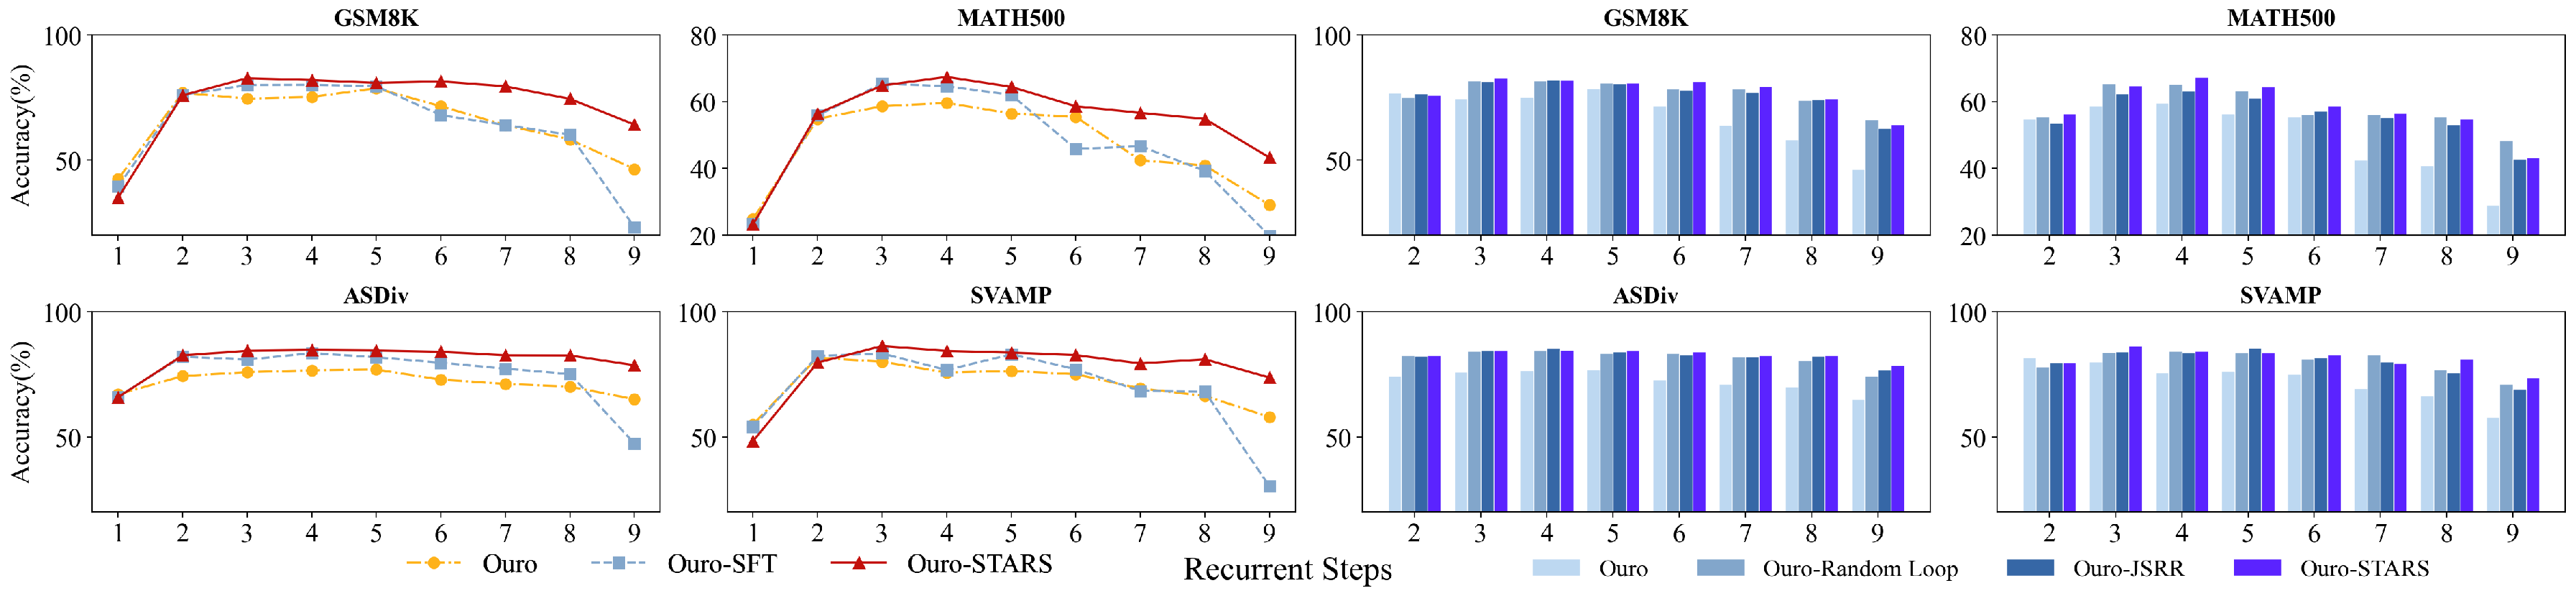
\includegraphics[width=\textwidth]{../papers/translations/stars/figures/ablation_with_compare.pdf}
\caption{原文图 4: 数学推理基准上, 本方法与基线及消融变体的比较. 左部展示 Ouro、Ouro-SFT 和 Ouro-STARS 的准确率随循环步数变化; 右部比较基础 Ouro、仅随机循环的 Ouro、仅 JSRR 的 Ouro 及 Ouro-STARS. 图内 Accuracy 为准确率, Recurrent Steps 为循环步数, Random Loop 为随机循环, JSRR 为 Jacobian 谱半径正则; 各小图标题保留基准名 GSM8K、MATH500、ASDiv、SVAMP.}\label{stars-fig-4}
\end{figure}
\begin{figure}[htbp]
\centering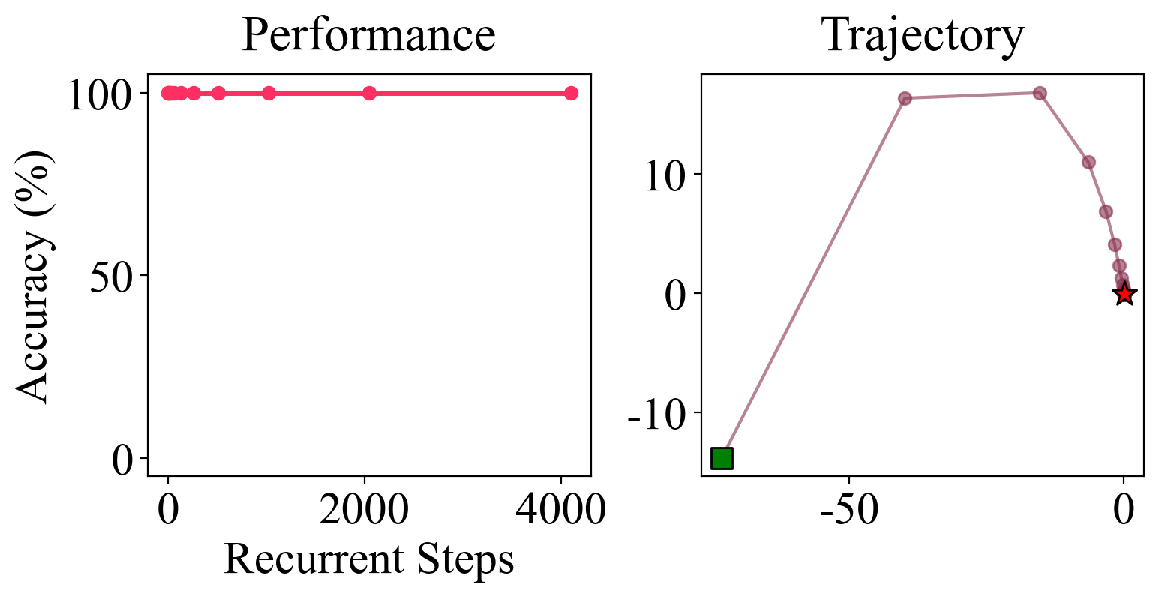
\includegraphics[width=.83\textwidth]{../papers/translations/stars/figures/main_addition.pdf}
\caption{原文图 5: 多位数加法上的性能与状态演化. 左部展示随循环步数变化的性能曲线, 反映模型稳定性; 右部为 PCA 投影后的隐状态动力学. Accuracy/Recurrent Steps 表示准确率/循环次数, Performance/Trajectory 为性能/轨迹; 轨迹坐标是前两主成分, 图中轨迹和曲线按原图保留.}\label{stars-fig-5}
\end{figure}

\noindent\textbf{实验设置.}\label{stars-sec-6-1}
\noindent\textbf{多位数加法任务.}
沿用前述实验设置, 根据已有发现使用 Post-Sandwich LayerNorm 结构. 随机循环配置采用对数正态采样, $\mu=2$, $\sigma=0.7$, 范围 $[1,100]$, 正则权重 $\lambda=0.1$. 训练学习率为 $1\times10^{-4}$.

\noindent\textbf{数学推理任务.}
基础模型为预训练循环语言模型 Ouro-1.4B\cite{stars-zhu2025scaling}, 针对其不可靠的测试时扩展行为. 受计算资源约束, 我们从 \texttt{NuminaMath-1.5}\cite{stars-li2024numinamath}随机取含 400K 样本的子集做微调. 配置为对数正态随机循环采样, $\mu=1.7$, $\sigma=0.4$, 范围 $[1,16]$, $\lambda=0.1$. 模型在四张 NVIDIA A800 GPU 上训练一个 epoch, 使用 AdamW\cite{stars-loshchilov2017decoupled}及从 $1\times10^{-6}$ 开始的余弦学习率调度. 然后使用 lm\_eval harness\cite{stars-eval-harness}, 在 GSM8K\cite{stars-cobbe2021gsm8k}、MATH500\cite{stars-lightman2023lets}、ASDiv\cite{stars-miao2020diverse}、SVAMP\cite{stars-patel2021nlp}、AMC23\cite{stars-yang2025qwen3}五个数学基准上做零样本评价.

\noindent\textbf{主要结果.}\label{stars-sec-6-2}
\noindent\textbf{多位数加法任务.}
如图 \ref{stars-fig-5}, 引入 STARS 后, 模型性能表现出明显鲁棒性. 无论循环迭代次数如何, 准确率保持 $100\%$, 表明模型稳定地学会了任务. 从动力系统角度看, 潜在状态以较快速度成功收敛到稳定不动点. 作者据此认为, 循环步数增加时仍可以可靠推理.

\noindent\textbf{数学推理任务.}
表 \ref{stars-tab-2} 汇总本框架、基础 Ouro-1.4B 和标准监督微调基线在五个数学基准上的表现, 还比较现有开放小模型. 与预期及既有循环模型观察一致, 超过名义训练深度时, 例如由 4 次循环增到 8 次, 基础模型与 SFT 基线都明显退化. SFT 平均准确率从 4 步的 $70.46\%$ 降到 8 步的 $52.97\%$.

相比之下, Ouro-1.4B-STARS 的分布内整体性能最好, 在 4 步达到平均准确率 $74.18\%$. 更关键的是, 扩展到 8 步时, 它仍维持 $65.55\%$ 的平均准确率. 如图 \ref{stars-fig-4} 右部所示, 随循环次数增加, 方法达到峰值后的下降更缓慢, 显示更稳定的扩展行为.

\noindent\textbf{消融研究.}\label{stars-sec-6-3}
为验证有效性并量化各组件的贡献, 我们在 GSM8K、MATH500、ASDiv、SVAMP 四个代表基准上进行消融. 比较基础 Ouro-1.4B, 以及三种变体: 只加入随机循环采样的 Ouro-Random Loop、只加入 JSRR 的 Ouro-JSRR、两者结合的完整 Ouro-STARS. 图 \ref{stars-fig-4} 右部表明, STARS 通常比各消融变体下降更慢; 随机循环采样和 JSRR 都有助于延缓退化. 更多分析见附录.

\originalsection{结论、影响声明与致谢}\label{stars-sec-7}
\noindent\textbf{结论.}
本文从动力系统视角发现并诊断当前 LoopLM 不可靠的扩展行为, 将其归因于推理有效性与潜在轨迹稳定性的内在权衡. 为解决这一问题, 我们提出 STARS, 一个将 Jacobian 谱半径正则化与随机循环采样结合、推动渐近稳定的统一训练框架. 合成任务与数学推理基准的实验表明, 相比先前方法, STARS 能在更大的循环深度上实现更可靠的测试时扩展.

\noindent\textbf{影响声明.}\label{stars-impact}
本文工作的目标是推进机器学习领域. 我们认为, 没有需要在此特别强调的潜在社会影响. 贡献主要在方法层面, 针对一类用于推理任务的循环语言模型架构, 改善其稳定性和扩展行为. 我们没有引入新应用或数据集, 也没有直接处理部署系统的公平性、安全性或偏见问题. 提出的技术在标准数学推理学术基准上评价.

\noindent\textbf{致谢.}\label{stars-acknowledgements}
研究得到江苏省科学基金(BK20243012, BG2024036, BK20232003)、国家自然科学基金(62576162), 以及中央高校基本科研业务费(022114380023)支持.

\originalsection{附录 A: 局限与未来工作}\paperlabel{A}{stars-app-A}
首先, 受计算资源约束, 实证评价集中在数学推理; 能否泛化到其他复杂推理领域, 如常识推理或策略规划, 仍是开放问题. 其次, 即使在这些任务上, STARS 虽然避免了灾难性崩溃, 并允许超过训练时域的扩展, 性能也并不总随步数增加而单调提高. 对最困难问题, 完全可靠且可预测的测试时扩展仍有挑战.

未来工作将把 STARS 扩展到更广的推理与规划任务, 并研究自适应机制, 以更稳健地引导潜在轨迹趋向最优、稳定的不动点.

\originalsection{附录 B: 训练算法细节}\paperlabel{B}{stars-app-B}
\noindent\textbf{原文算法 1: 使用 JSRR 训练循环语言模型的 STARS.}\label{stars-alg-1}
输入为数据集 $\mathcal D$, 初始参数 $\theta$, 分布 $\mathcal P$, 正则权重 $\lambda$, 学习率 $\eta$, 幂迭代步数 $K$.
\begin{enumerate}
\item 重复下列过程, 直到收敛.
\item 从 $\mathcal D$ 采样一个批次 $\{\mathbf x^{(i)},\mathbf y^{(i)}\}_{i=1}^N$; 采样循环深度 $t\sim\mathcal P$.
\item 对每个 $i=1,\ldots,N$, 先向前运行到循环深度 $t$:
\[
\mathbf h_i^{(0)}\gets\operatorname{prelude}(\mathbf x^{(i)}),\qquad
\mathbf h_i^{(t)}\gets\underbrace{\Phi_\theta\circ\cdots\circ\Phi_\theta}_{t\text{ 次}}(\mathbf h_i^{(0)}).
\]
\item 对这个样本初始化随机方向:
\[
\mathbf v^{(i)}\sim\mathcal N(0,I),\qquad
\mathbf v^{(i)}\gets\frac{\mathbf v^{(i)}}{\|\mathbf v^{(i)}\|_2+\epsilon}.
\]
\item 对 $k=1,\ldots,K$, 用 Jacobian--向量积做幂迭代:
\begin{align*}
\mathbf j^{(i)}&\gets\operatorname{JVP}(\Phi_\theta,\mathbf h_i^{(t)},\mathbf v^{(i)}),\\
\mathbf v^{(i)}&\gets\frac{\mathbf j^{(i)}}{\|\mathbf j^{(i)}\|_2+\epsilon}.
\end{align*}
循环结束后, 令 $\mathcal L_{\rm JSRR}^{(i)}\gets\|\mathbf j^{(i)}\|_2^2$. 这一步完成该样本的计算; 对其余样本重复以上操作.
\item 计算损失:
\begin{align*}
\mathcal L_{\rm SFT}^{(t)}&\gets\frac1N\sum_{i=1}^N-\log p_\theta^{(t)}(\mathbf y^{(i)}\mid\mathbf x^{(i)}),\\
\mathcal L_{\rm JSRR}^{(t)}&\gets\frac1N\sum_{i=1}^N\mathcal L_{\rm JSRR}^{(i)},\\
\mathcal L&\gets\mathcal L_{\rm SFT}^{(t)}+\lambda\mathcal L_{\rm JSRR}^{(t)}.
\end{align*}
\item 优化一步: $\theta\gets\theta-\eta\nabla_\theta\mathcal L$, 然后进入下一次重复.
\end{enumerate}

\originalsection{附录 C: 更多结果}\paperlabel{C}{stars-app-C}
\noindent\textbf{PreNorm 与 PostNorm 上的随机循环采样.}\label{stars-app-C-1}
我们补充了使用 LN 的 PreNorm 和 PostNorm 在对数正态、泊松、均匀三种分布下的随机循环结果, 每种分布两组配置, 见图 \ref{stars-fig-6} 与表 \ref{stars-tab-3}.
\begin{figure}[htbp]
\centering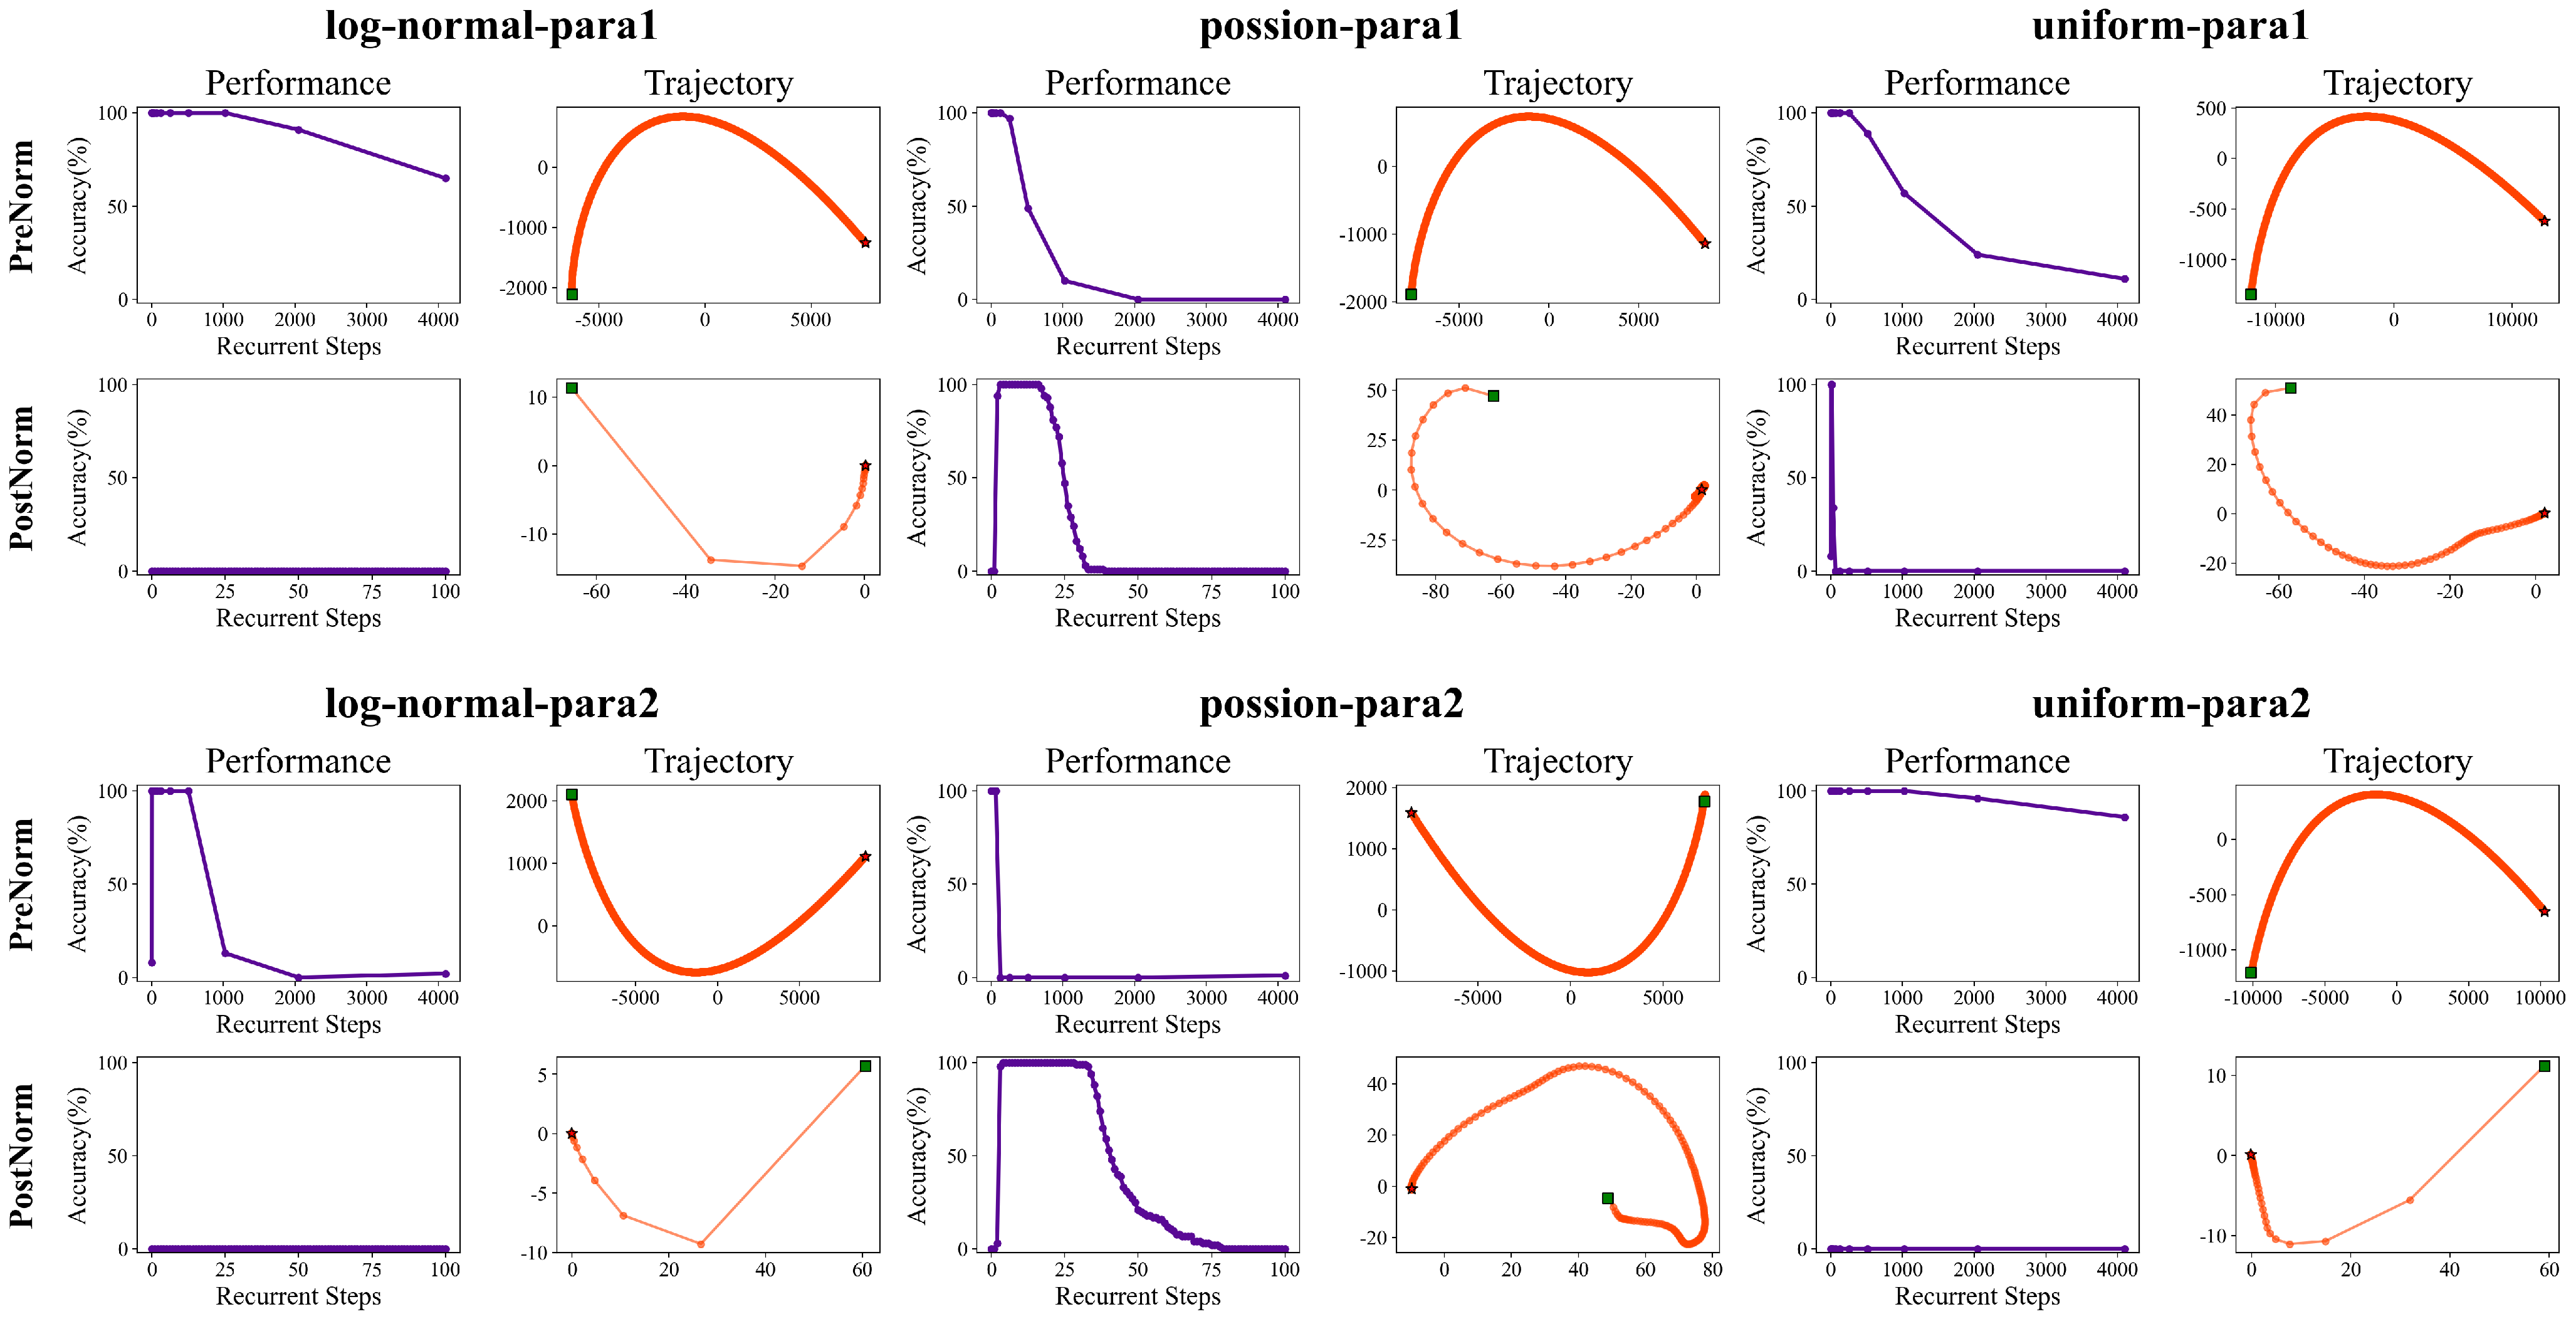
\includegraphics[width=\textwidth]{../papers/translations/stars/figures/pre_post_random.pdf}
\caption{原文图 6: PreNorm 与 PostNorm 使用 LN 时, 不同分布和参数组下的随机循环策略结果. 图内 PreNorm/PostNorm 为前置/后置归一化, LN 为 LayerNorm; Log-Normal/Poisson/Uniform 是对数正态/泊松/均匀分布, para1/para2 为两参数组, Accuracy/Recurrent Steps 为准确率/循环次数, Performance/Trajectory 为性能/轨迹, 其余为 PCA 潜在轨迹.}\label{stars-fig-6}
\end{figure}
\begin{table}[htbp]
\centering
\caption{原文表 3: PreNorm 与 PostNorm 的随机循环分布超参数. 范围是截断边界 $[\min,\max]$.}\label{stars-tab-3}
\begin{tabular}{lll}\toprule
分布 & 参数组 1 & 参数组 2\\\midrule
对数正态 & $\mu=2.62$, $\sigma=0.60$ & $\mu=3.2$, $\sigma=0.45$\\
 & 范围 $[1,40]$ & 范围 $[1,80]$\\
泊松 & $\lambda=5$ & $\lambda=10$\\
 & 范围 $[1,30]$ & 范围 $[1,30]$\\
均匀 & 范围 $[1,10]$ & 范围 $[1,30]$\\\bottomrule
\end{tabular}
\end{table}

\noindent\textbf{超参数分析.}\label{stars-app-C-2}
我们在多位数加法任务上分析正则权重 $\lambda$, 结果见图 \ref{stars-fig-7}. 对一系列 $\lambda$ 值, 绘制性能曲线和 PCA 投影轨迹. $\lambda$ 直接决定 JSRR 约束强度, 并反映在潜在动力学中. 不同权重均能让模型趋向吸引子, 但权重过大, 如 $0.15$ 和 $0.20$, 会使模型难以学会原多位数任务, 性能曲线的准确率明显下降. 因此, 方法虽有一定鲁棒性, 正则权重不应过大, 否则阻碍有效学习.
\begin{figure}[htbp]
\centering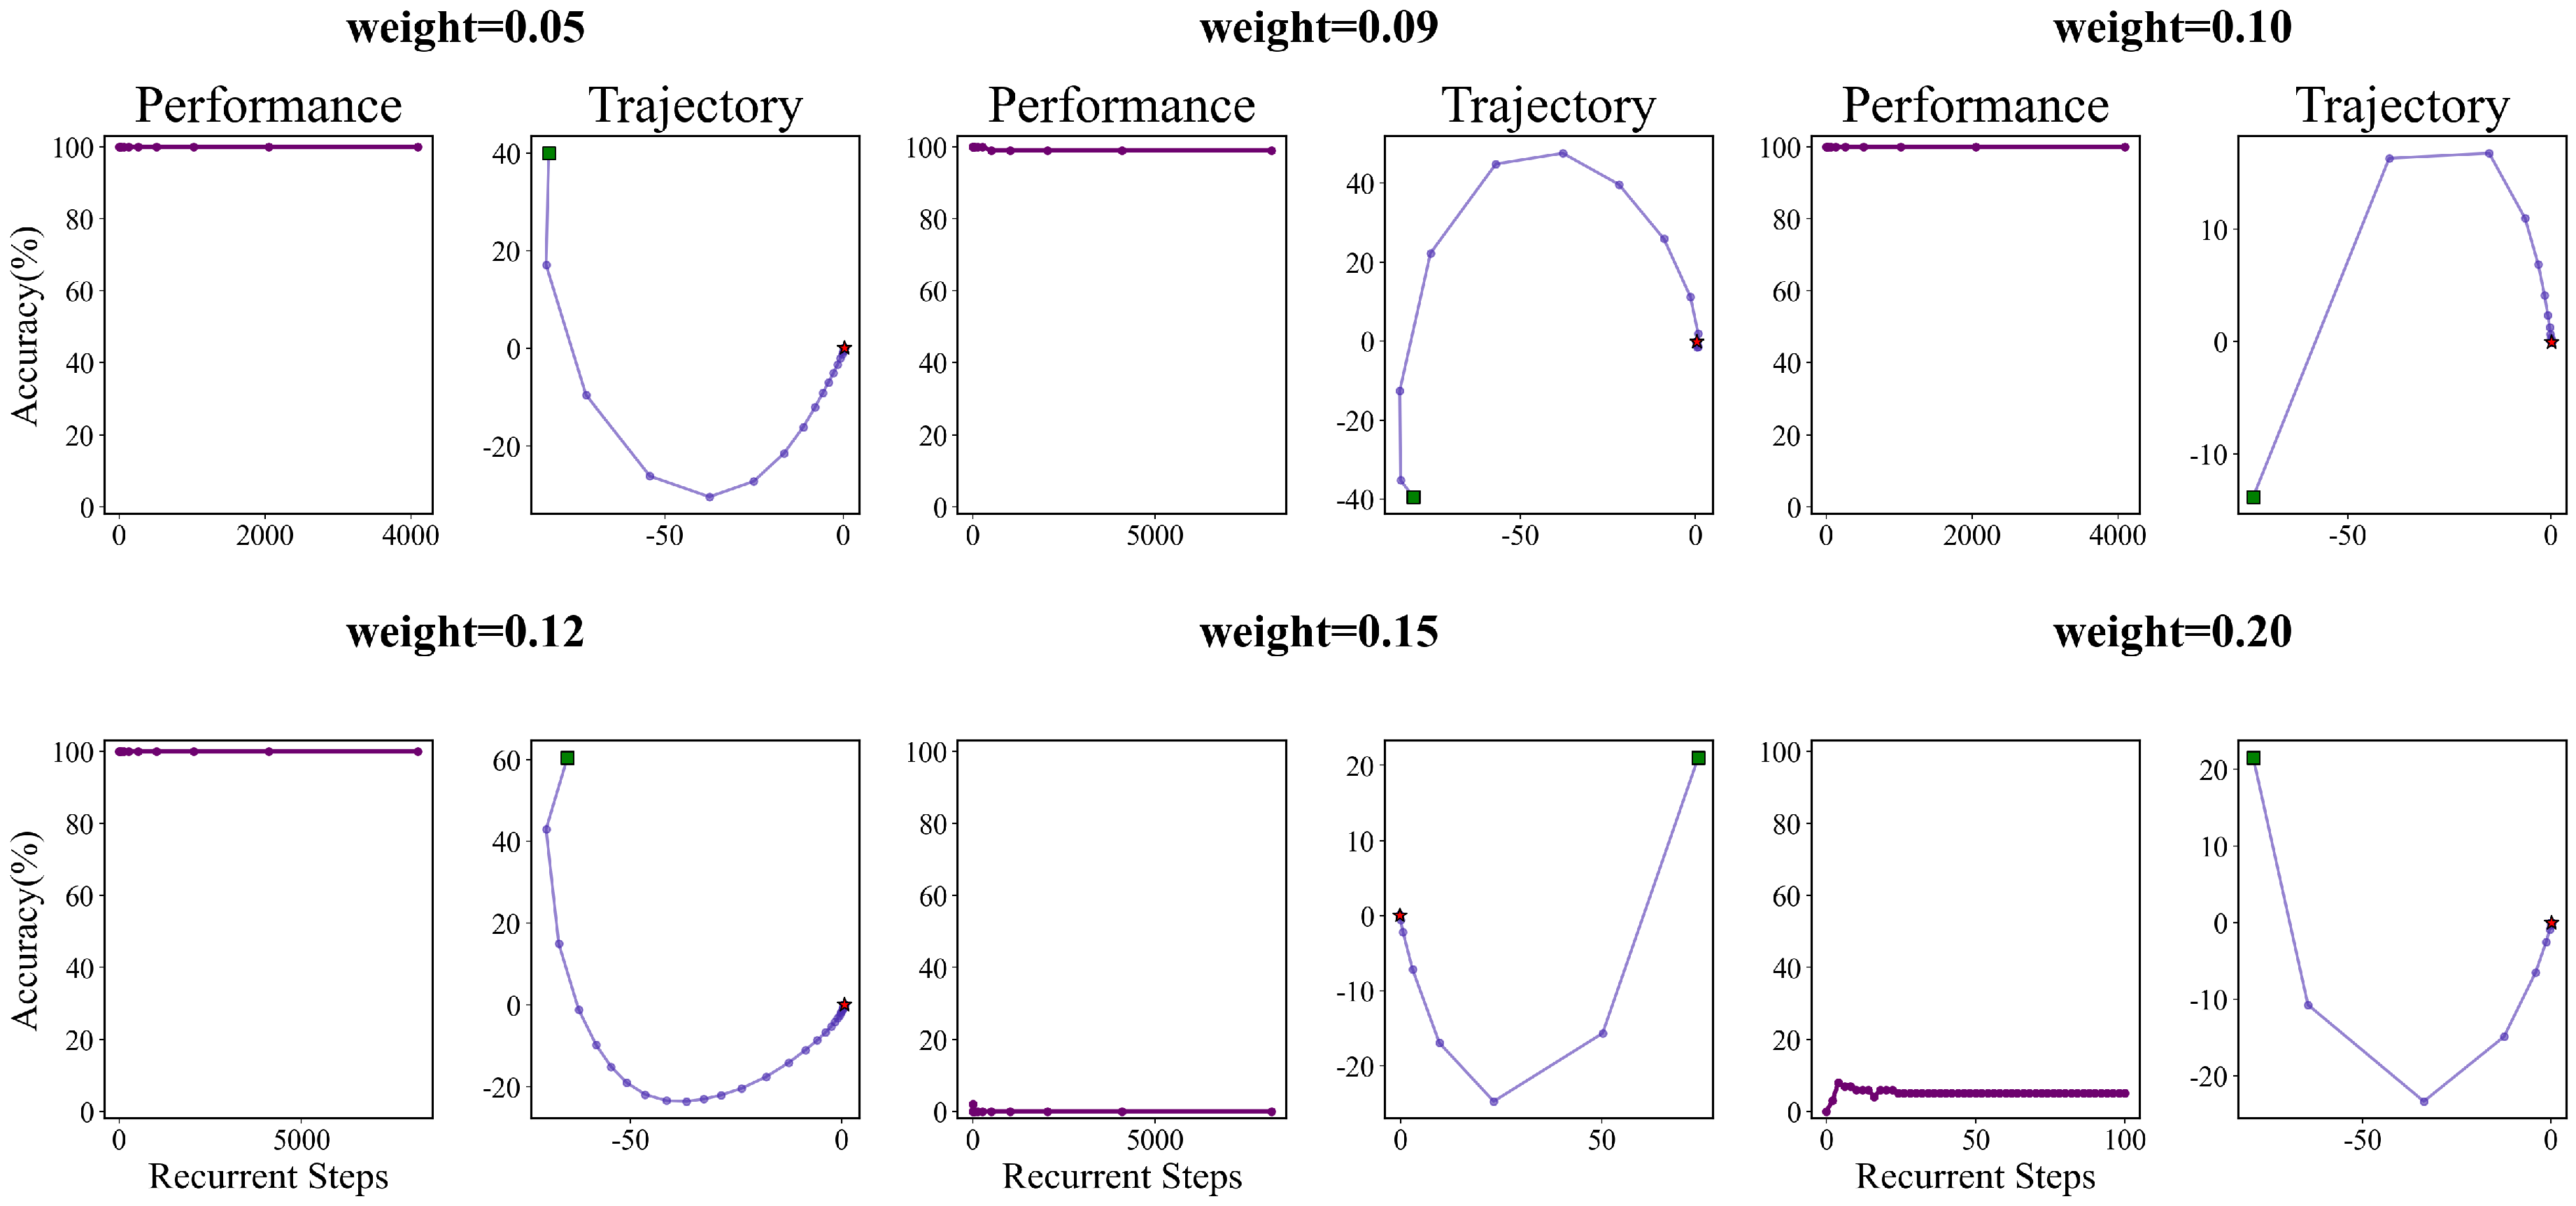
\includegraphics[width=.96\textwidth]{../papers/translations/stars/figures/weight.pdf}
\caption{原文图 7: 多位数加法任务的超参数分析. $\lambda$ 为正则权重, 图内 weight 为权重; Accuracy/Recurrent Steps 表示准确率/循环次数, Performance/Trajectory 为性能/轨迹. 图中同时展示不同权重的性能曲线及 PCA 状态轨迹.}\label{stars-fig-7}
\end{figure}

\noindent\textbf{训练阶段效率分析.}\label{stars-app-C-3}
我们以 Ouro-SFT 为基线, 分析四类配置的训练阶段效率. 结果见表 \ref{stars-tab-4}. 相对于 Ouro-SFT, Ouro-Random Loop、Ouro-JSRR、Ouro-STARS 的训练阶段相对值分别为 $1.4976$, $1.5317$, $2.0439$.
\begin{table}[htbp]
\centering
\caption{原文表 4: 训练阶段效率分析, 数值均以 Ouro-SFT 为基准.}\label{stars-tab-4}
\begin{tabular}{lr}\toprule
模型 & 相对值\\\midrule
Ouro-SFT & 1\\
Ouro-Random Loop & 1.4976\\
Ouro-JSRR & 1.5317\\
Ouro-STARS & 2.0439\\\bottomrule
\end{tabular}
\end{table}

\noindent\textbf{AMC23 上的比较与消融.}\label{stars-app-C-4}
除正文图 \ref{stars-fig-4} 的数学基准分析外, 我们还在 AMC23 数据集比较方法、基线及消融变体, 结果见图 \ref{stars-fig-8}.
\begin{figure}[htbp]
\centering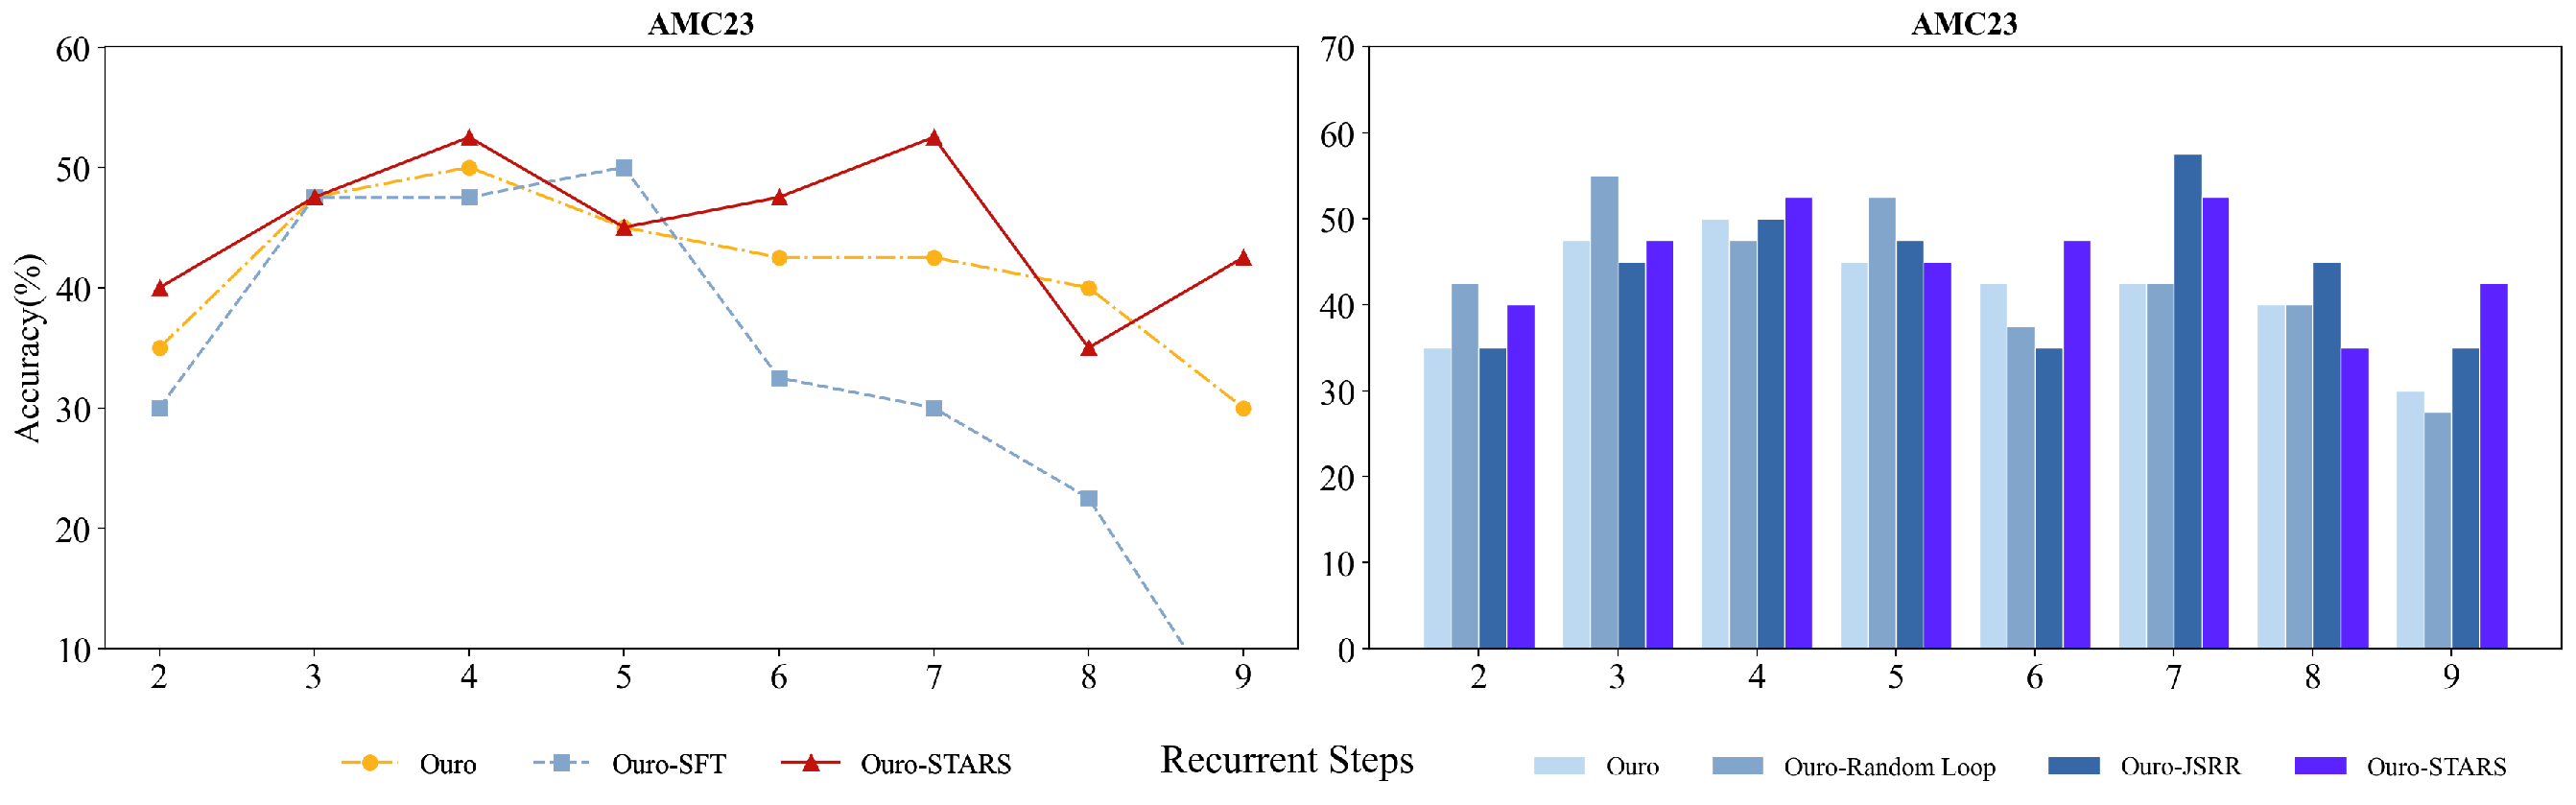
\includegraphics[width=\textwidth]{../papers/translations/stars/figures/amc23_ablation.pdf}
\caption{原文图 8: AMC23 上, 本方法与基线及消融变体的比较. Accuracy/Recurrent Steps 表示准确率/循环步数; Ouro、Ouro-SFT、Ouro-STARS 与仅 Random Loop、仅 JSRR 的变体对应正文相同配置.}\label{stars-fig-8}
\end{figure}

\originalsection{译者核查注}\label{stars-translator-notes}
本节为译者补充, 不属于作者论文. 全文保留原文的实验报告和方法主张; 下列差异没有被静默修正.

第一, 局部线性化结论讨论已存在不动点附近的光滑动力系统. 当前状态处的正则、有限样本上的谱估计及随机循环训练, 不自动证明全部输入轨迹都存在稳定不动点, 更不证明其读出语义正确. 原文“保证”“全局稳定性”等较强措辞应连同方法的代理性质及附录 A 的限制阅读.

第二, 幂迭代趋向主特征向量需要额外谱条件及合适初始方向. 单步 $\|Jv\|_2$ 一般不是谱半径的精确或无偏估计. 若忽略算法中的 $\epsilon$, 并将 $v$ 取为均匀随机单位向量, 则 $\E\|Jv\|_2^2=\|J\|_F^2/D$, 这是平均方向伸长的量, 并非一般矩阵的 $\rho(J)^2$. 原文“跨批次统计方向准确”的说法没有附上相应证明. 对非正规矩阵, 谱半径小也不排除短期扰动放大.

第三, 正文总目标为式 \eqref{stars-eq-4} 的 $(1-\lambda)\mathcal L_{\rm SFT}+\lambda\mathcal L_{\rm JSRR}$, 算法却写 $\mathcal L_{\rm SFT}+\lambda\mathcal L_{\rm JSRR}$. 若 $0<\lambda<1$, 乘去整体常数后, 前者相对正则权重是 $\lambda/(1-\lambda)$, 与算法同名 $\lambda$ 不同. 本译稿保留两处原写法. 正文式 \eqref{stars-eq-3} 写 $v$, 后文说明写 $v_1$, 也保留这一记号差异.

第四, 随机循环段落将 Pre-Sandwich 后的漂移归于“外部归一化系统”, 与本论文前面的内部/外部分类不一致; 本译稿用“原文称”保留并提示. 引言写状态“指数”增长, 后文诊断写“线性”放大, 两处没有被统一. 原文一般地称不动点为吸引子, 但不动点也可能不稳定; 标准意义上的局部渐近稳定还通常包含 Lyapunov 稳定性, 不只吸引性. 译稿保留原定义, 不将它悄悄增强成完整定理.

第五, 引言的 $20.47\%$, $8.26\%$, $4.01\%$ 原文未清楚注明相对百分比或百分点, 且表 \ref{stars-tab-2} 中 Ouro 峰值 $76.88$ 到 8 步 $58.23$ 的差为 $18.65$ 个百分点; STARS 峰值 $81.96$ 到 $74.45$ 的差为 $7.51$ 个百分点. 引言数值与主表不能直接互相恢复. 本译稿保留引言和主表全部原数字, 不自行选择其中一组替换. 表 \ref{stars-tab-4} 只标示相对效率值, 未在该表定义是耗时、成本还是吞吐, 所以没有译成“加速倍数”.

% 原论文实际生成的完整41项书目;作者、题名与出版信息保留原文以便检索.
\begin{thebibliography}{41}
\providecommand{\natexlab}[1]{#1}
\providecommand{\url}[1]{\texttt{#1}}
\expandafter\ifx\csname urlstyle\endcsname\relax
  \providecommand{\doi}[1]{doi: #1}\else
  \providecommand{\doi}{doi: \begingroup \urlstyle{rm}\Url}\fi

\bibitem{stars-ba2016layer}
Ba, J.~L., Kiros, J.~R., and Hinton, G.~E.
\newblock Layer normalization.
\newblock \textit{arXiv preprint arXiv:1607.06450}, 2016.

\bibitem{stars-bai2019deep}
Bai, S., Kolter, J.~Z., and Koltun, V.
\newblock Deep equilibrium models.
\newblock \textit{Advances in neural information processing systems}, 32, 2019.

\bibitem{stars-bai2021stabilizing}
Bai, S., Koltun, V., and Kolter, J.~Z.
\newblock Stabilizing equilibrium models by jacobian regularization.
\newblock \textit{arXiv preprint arXiv:2106.14342}, 2021.

\bibitem{stars-cheng2024compressed}
Cheng, J. and Van~Durme, B.
\newblock Compressed chain of thought: Efficient reasoning through dense
  representations.
\newblock \textit{arXiv preprint arXiv:2412.13171}, 2024.

\bibitem{stars-cobbe2021gsm8k}
Cobbe, K., Kosaraju, V., Bavarian, M., Chen, M., Jun, H., Kaiser, L., Plappert,
  M., Tworek, J., Hilton, J., Nakano, R., Hesse, C., and Schulman, J.
\newblock Training verifiers to solve math word problems.
\newblock \textit{arXiv preprint arXiv:2110.14168}, 2021.

\bibitem{stars-dehghani2018universal}
Dehghani, M., Gouws, S., Vinyals, O., Uszkoreit, J., and Kaiser, {\L}.
\newblock Universal transformers.
\newblock \textit{arXiv preprint arXiv:1807.03819}, 2018.

\bibitem{stars-du2025latent}
Du, H., Dong, Y., and Ning, X.
\newblock Latent thinking optimization: Your latent reasoning language model
  secretly encodes reward signals in its latent thoughts.
\newblock \textit{arXiv preprint arXiv:2509.26314}, 2025.

\bibitem{stars-fan2024looped}
Fan, Y., Du, Y., Ramchandran, K., and Lee, K.
\newblock Looped transformers for length generalization.
\newblock \textit{arXiv preprint arXiv:2409.15647}, 2024.

\bibitem{stars-eval-harness}
Gao, L., Tow, J., Abbasi, B., Biderman, S., Black, S., DiPofi, A., Foster, C.,
  Golding, L., Hsu, J., Le~Noac'h, A., Li, H., McDonell, K., Muennighoff, N.,
  Ociepa, C., Phang, J., Reynolds, L., Schoelkopf, H., Skowron, A., Sutawika,
  L., Tang, E., Thite, A., Wang, B., Wang, K., and Zou, A.
\newblock The language model evaluation harness, 07 2024.

\bibitem{stars-geiping2025scaling}
Geiping, J., McLeish, S., Jain, N., Kirchenbauer, J., Singh, S., Bartoldson,
  B.~R., Kailkhura, B., Bhatele, A., and Goldstein, T.
\newblock Scaling up test-time compute with latent reasoning: A recurrent depth
  approach.
\newblock \textit{arXiv preprint arXiv:2502.05171}, 2025.

\bibitem{stars-giannou2023looped}
Giannou, A., Rajput, S., Sohn, J.-y., Lee, K., Lee, J.~D., and Papailiopoulos,
  D.
\newblock Looped transformers as programmable computers.
\newblock In \textit{International Conference on Machine Learning}, pp.\
  11398--11442. PMLR, 2023.

\bibitem{stars-grattafiori2024llama}
Grattafiori, A., Dubey, A., Jauhri, A., Pandey, A., Kadian, A., Al-Dahle, A.,
  Letman, A., Mathur, A., Schelten, A., Vaughan, A., et~al.
\newblock The llama 3 herd of models.
\newblock \textit{arXiv preprint arXiv:2407.21783}, 2024.

\bibitem{stars-hao2024training}
Hao, S., Sukhbaatar, S., Su, D., Li, X., Hu, Z., Weston, J., and Tian, Y.
\newblock Training large language models to reason in a continuous latent
  space.
\newblock \textit{arXiv preprint arXiv:2412.06769}, 2024.

\bibitem{stars-he2016deep}
He, K., Zhang, X., Ren, S., and Sun, J.
\newblock Deep residual learning for image recognition.
\newblock In \textit{Proceedings of the IEEE conference on computer vision and
  pattern recognition}, pp.\  770--778, 2016.

\bibitem{stars-li2024numinamath}
Li, J., Beeching, E., Tunstall, L., Lipkin, B., Soletskyi, R., Huang, S.,
  Rasul, K., Yu, L., Jiang, A.~Q., Shen, Z., et~al.
\newblock Numinamath: The largest public dataset in ai4maths with 860k pairs of
  competition math problems and solutions.
\newblock \textit{Hugging Face repository}, 13\penalty0 (9):\penalty0 9, 2024.

\bibitem{stars-lightman2023lets}
Lightman, H., Kosaraju, V., Burda, Y., Edwards, H., Baker, B., Lee, T., Leike,
  J., Schulman, J., Sutskever, I., and Cobbe, K.
\newblock Let's verify step by step.
\newblock \textit{arXiv preprint arXiv:2305.20050}, 2023.

\bibitem{stars-loshchilov2017decoupled}
Loshchilov, I. and Hutter, F.
\newblock Decoupled weight decay regularization.
\newblock \textit{arXiv preprint arXiv:1711.05101}, 2017.

\bibitem{stars-mcleish2025teaching}
McLeish, S., Li, A., Kirchenbauer, J., Kalra, D.~S., Bartoldson, B.~R.,
  Kailkhura, B., Schwarzschild, A., Geiping, J., Goldstein, T., and Goldblum,
  M.
\newblock Teaching pretrained language models to think deeper with retrofitted
  recurrence.
\newblock \textit{arXiv preprint arXiv:2511.07384}, 2025.

\bibitem{stars-miao2020diverse}
Miao, S.-Y., Liang, C.-C., and Su, K.-Y.
\newblock A diverse corpus for evaluating and developing english math word
  problem solvers.
\newblock In \textit{Proceedings of the 58th annual meeting of the Association
  for Computational Linguistics}, pp.\  975--984, 2020.

\bibitem{stars-mohtashami2023cotformer}
Mohtashami, A., Pagliardini, M., and Jaggi, M.
\newblock Cotformer: A chain-of-thought driven architecture with
  budget-adaptive computation cost at inference.
\newblock \textit{arXiv preprint arXiv:2310.10845}, 2023.

\bibitem{stars-patel2021nlp}
Patel, A., Bhattamishra, S., and Goyal, N.
\newblock Are nlp models really able to solve simple math word problems?
\newblock \textit{arXiv preprint arXiv:2103.07191}, 2021.

\bibitem{stars-radford2019language}
Radford, A., Wu, J., Child, R., Luan, D., Amodei, D., Sutskever, I., et~al.
\newblock Language models are unsupervised multitask learners.
\newblock \textit{OpenAI blog}, 1\penalty0 (8):\penalty0 9, 2019.

\bibitem{stars-shen2025codi}
Shen, Z., Yan, H., Zhang, L., Hu, Z., Du, Y., and He, Y.
\newblock Codi: Compressing chain-of-thought into continuous space via
  self-distillation.
\newblock \textit{arXiv preprint arXiv:2502.21074}, 2025.

\bibitem{stars-team2025gemma}
Team, G., Kamath, A., Ferret, J., Pathak, S., Vieillard, N., Merhej, R.,
  Perrin, S., Matejovicova, T., Ram{\'e}, A., Rivi{\`e}re, M., et~al.
\newblock Gemma 3 technical report.
\newblock \textit{arXiv preprint arXiv:2503.19786}, 2025.

\bibitem{stars-team2024qwen2}
Team, Q. et~al.
\newblock Qwen2 technical report.
\newblock \textit{arXiv preprint arXiv:2407.10671}, 2\penalty0 (3), 2024.

\bibitem{stars-vaswani2017attention}
Vaswani, A., Shazeer, N., Parmar, N., Uszkoreit, J., Jones, L., Gomez, A.~N.,
  Kaiser, {\L}., and Polosukhin, I.
\newblock Attention is all you need.
\newblock \textit{Advances in neural information processing systems}, 30, 2017.

\bibitem{stars-wang2022selfconsistency}
Wang, X., Wei, J., Schuurmans, D., Le, Q., Chi, E., Narang, S., Chowdhery, A.,
  and Zhou, D.
\newblock Self-consistency improves chain of thought reasoning in language
  models.
\newblock \textit{International Conference on Learning Representations}, 2022.

\bibitem{stars-wei2022chain}
Wei, J., Wang, X., Schuurmans, D., Bosma, M., Xia, F., Chi, E., Le, Q.~V.,
  Zhou, D., et~al.
\newblock Chain-of-thought prompting elicits reasoning in large language
  models.
\newblock \textit{Advances in neural information processing systems},
  35:\penalty0 24824--24837, 2022.

\bibitem{stars-wei2025sim}
Wei, X., Liu, X., Zang, Y., Dong, X., Cao, Y., Wang, J., Qiu, X., and Lin, D.
\newblock Sim-cot: Supervised implicit chain-of-thought.
\newblock \textit{arXiv preprint arXiv:2509.20317}, 2025.

\bibitem{stars-xiong2020layer}
Xiong, R., Yang, Y., He, D., Zheng, K., Zheng, S., Xing, C., Zhang, H., Lan,
  Y., Wang, L., and Liu, T.
\newblock On layer normalization in the transformer architecture.
\newblock In \textit{International conference on machine learning}, pp.\
  10524--10533. PMLR, 2020.

\bibitem{stars-yang2025qwen3}
Yang, A., Li, A., Yang, B., Zhang, B., Hui, B., Zheng, B., Yu, B., Gao, C.,
  Huang, C., Lv, C., et~al.
\newblock Qwen3 technical report.
\newblock \textit{arXiv preprint arXiv:2505.09388}, 2025.

\bibitem{stars-yang2023looped}
Yang, L., Lee, K., Nowak, R., and Papailiopoulos, D.
\newblock Looped transformers are better at learning learning algorithms.
\newblock \textit{arXiv preprint arXiv:2311.12424}, 2023.

\bibitem{stars-yang2022chain}
Yang, M.~S., Schuurmans, D., Abbeel, P., and Nachum, O.
\newblock Chain of thought imitation with procedure cloning.
\newblock \textit{Advances in Neural Information Processing Systems}, pp.\
  36366--36381, 2022.

\bibitem{stars-tot}
Yao, S., Yu, D., Zhao, J., Shafran, I., Griffiths, T., Cao, Y., and Narasimhan,
  K.
\newblock Tree of thoughts: Deliberate problem solving with large language
  models.
\newblock \textit{Advances in Neural Information Processing Systems}, 2024.

\bibitem{stars-zelikman2024quiet}
Zelikman, E., Harik, G., Shao, Y., Jayasiri, V., Haber, N., and Goodman, N.~D.
\newblock Quiet-star: Language models can teach themselves to think before
  speaking.
\newblock \textit{arXiv preprint arXiv:2403.09629}, 2024.

\bibitem{stars-zhang2019root}
Zhang, B. and Sennrich, R.
\newblock Root mean square layer normalization.
\newblock \textit{Advances in neural information processing systems}, 32, 2019.

\bibitem{stars-zhang2025lightthinker}
Zhang, J., Zhu, Y., Sun, M., Luo, Y., Qiao, S., Du, L., Zheng, D., Chen, H.,
  and Zhang, N.
\newblock Lightthinker: Thinking step-by-step compression.
\newblock \textit{arXiv preprint arXiv:2502.15589}, 2025{\natexlab{a}}.

\bibitem{stars-zhang2025survey}
Zhang, Q., Lyu, F., Sun, Z., Wang, L., Zhang, W., Hua, W., Wu, H., Guo, Z.,
  Wang, Y., Muennighoff, N., et~al.
\newblock A survey on test-time scaling in large language models: What, how,
  where, and how well?
\newblock \textit{arXiv preprint arXiv:2503.24235}, 2025{\natexlab{b}}.

\bibitem{stars-zhang2024llm}
Zhang, Y., Mao, S., Ge, T., Wang, X., de~Wynter, A., Xia, Y., Wu, W., Song, T.,
  Lan, M., and Wei, F.
\newblock Llm as a mastermind: A survey of strategic reasoning with large
  language models.
\newblock \textit{arXiv preprint arXiv:2404.01230}, 2024.

\bibitem{stars-zhu2025survey}
Zhu, R.-J., Peng, T., Cheng, T., Qu, X., Huang, J., Zhu, D., Wang, H., Xue, K.,
  Zhang, X., Shan, Y., et~al.
\newblock A survey on latent reasoning.
\newblock \textit{arXiv preprint arXiv:2507.06203}, 2025{\natexlab{a}}.

\bibitem{stars-zhu2025scaling}
Zhu, R.-J., Wang, Z., Hua, K., Zhang, T., Li, Z., Que, H., Wei, B., Wen, Z.,
  Yin, F., Xing, H., et~al.
\newblock Scaling latent reasoning via looped language models.
\newblock \textit{arXiv preprint arXiv:2510.25741}, 2025{\natexlab{b}}.

\end{thebibliography}

